% mnras_template.tex
%
% LaTeX template for creating an MNRAS paper
%
% v3.0 released 14 May 2015
% (version numbers match those of mnras.cls)
%
% Copyright (C) Royal Astronomical Society 2015
% Authors:
% Keith T. Smith (Royal Astronomical Society)

% Change log
%
% v3.0 May 2015
%    Renamed to match the new package name
%    Version number matches mnras.cls
%    A few minor tweaks to wording
% v1.0 September 2013
%    Beta testing only - never publicly released
%    First version: a simple (ish) template for creating an MNRAS paper

%%%%%%%%%%%%%%%%%%%%%%%%%%%%%%%%%%%%%%%%%%%%%%%%%%
% Basic setup. Most papers should leave these options alone.
\documentclass[a4paper,fleqn,usenatbib]{mnras}

% MNRAS is set in Times font. If you don't have this installed (most LaTeX
% installations will be fine) or prefer the old Computer Modern fonts, comment
% out the following line
\usepackage{newtxtext,newtxmath}
% Depending on your LaTeX fonts installation, you might get better results with one of these:
%\usepackage{mathptmx}
%\usepackage{txfonts}

% Use vector fonts, so it zooms properly in on-screen viewing software
% Don't change these lines unless you know what you are doing
\usepackage[T1]{fontenc}
\usepackage{ae,aecompl}


%%%%% AUTHORS - PLACE YOUR OWN PACKAGES HERE %%%%%

% Only include extra packages if you really need them. Common packages are:
\usepackage{graphicx}	% Including figure files
\usepackage{amsmath}	% Advanced maths commands
\usepackage{amssymb}	% Extra maths symbols
\usepackage{pdflscape}

%%%%%%%%%%%%%%%%%%%%%%%%%%%%%%%%%%%%%%%%%%%%%%%%%%

%%%%% AUTHORS - PLACE YOUR OWN COMMANDS HERE %%%%%

% Please keep new commands to a minimum, and use \newcommand not \def to avoid
% overwriting existing commands. Example:
%\newcommand{\pcm}{\,cm$^{-2}$}	% per cm-squared

%%%%%%%%%%%%%%%%%%%%%%%%%%%%%%%%%%%%%%%%%%%%%%%%%%

%%%%%%%%%%%%%%%%%%% TITLE PAGE %%%%%%%%%%%%%%%%%%%

\usepackage{xspace}
\newcommand{\geu}{iPTF16geu\xspace}
\newcommand{\scipap}{G17\xspace}
\newcommand{\sn}{SN\xspace}
\newcommand{\snia}{SN~Ia\xspace}
\newcommand{\sneia}{SNe~Ia\xspace}
\newcommand{\sne}{SNe\xspace}
\newcommand{\hst}{HST\xspace}
\newcommand{\wfc}{WFC3\xspace}
\newcommand{\uvis}{UVIS\xspace}
\newcommand{\ir}{IR\xspace}
\newcommand{\wfcuvis}{WFC3/UVIS\xspace}
\newcommand{\wfcir}{WFC3/IR\xspace}
\newcommand{\uvisaperture}{{\tt UVIS2-C512C-SUB}\xspace}
\newcommand{\iraperture}{{\tt IRSUB512}\xspace}
\newcommand{\jband}{{\it J}\xspace}
\newcommand{\hband}{{\it H}\xspace}
\newcommand{\ksband}{{\it Ks}\xspace}
\newcommand{\hstu}{$F390W$\xspace}
\newcommand{\hstb}{$F475W$\xspace}
\newcommand{\hstr}{$F625W$\xspace}
\newcommand{\hsti}{$F814W$\xspace}
\newcommand{\hstj}{$F110W$\xspace}
\newcommand{\hsth}{$F160W$\xspace}

\newcommand{\sd}[1]{\textcolor{green}{SD: #1}}

% Title of the paper, and the short title which is used in the headers.
% Keep the title short and informative.
\title[Extinction and time-delay constraints from \geu]{Extinction and time-delay constraints from the first resolved strongly lensed Type Ia supernova \geu}

% The list of authors, and the short list which is used in the headers.
% If you need two or more lines of authors, add an extra line using \newauthor
\author[Amanullah et al.]{%
R.~Amanullah,$^{1}$\thanks{E-mail: rahman@fysik.su.se}
A.~Goobar,$^{1}$
B.~Cenko,
A.~Cooray,
O.~Fox,
R.~Kalender,$^{1}$
\newauthor
M.~Kasliwal,
E.~M\"ortsell,$^{1}$
H.~Nayyeri
\\
% List of institutions
$^{1}$The Oskar Klein Centre, Physics Department,
    Stockholm University,
    Albanova University Center, SE 106 91 Stockholm, Sweden\\
}

% These dates will be filled out by the publisher
\date{Accepted XXX. Received YYY; in original form ZZZ}

% Enter the current year, for the copyright statements etc.
\pubyear{2017}

% Don't change these lines
\begin{document}
\label{firstpage}
\pagerange{\pageref{firstpage}--\pageref{lastpage}}
\maketitle

% Abstract of the paper
\begin{abstract}
Observations of resolved strongly lensed Type Ia supernovae (\sneia) can be used for cosmological applications or to study
properties of the lensing galaxy, such as extinction and the matter distribution .  Here we report the results from 
measurements obtained with the Hubble Space Telescope of the multiple images of \geu.
\end{abstract}
%hej hej
% Select between one and six entries from the list of approved keywords.
% Don't make up new ones.
\begin{keywords}
keyword1 -- keyword2 -- keyword3
\end{keywords}

%%%%%%%%%%%%%%%%%%%%%%%%%%%%%%%%%%%%%%%%%%%%%%%%%%

%%%%%%%%%%%%%%%%% BODY OF PAPER %%%%%%%%%%%%%%%%%%

\section{Introduction}
More than half a century has passed since
\citet{1964MNRAS.128..307R} proposed  to measure the expansion rate of the universe, the Hubble parameter, using time delay measurements of multiply-imaged gravitationally lensed supernovae (\sne). However, discovering these rare events has proven very challenging and it is only thanks to 
the recent developments in time domain astronomy that the first couple of resolved lensed supernovae have been detected. SN Refsdal \citep{2015Sci...347.1123K}, detected with the Hubble Space Telescope (HST), is a core-collapse \sn magnified by a cluster of galaxies, while 
iPTF16geu \citep{2017Sci...356..291G}, the subject of this work, is split into four resolved images by an individual galaxy. Furthermore, it was spectroscopically classified as a Type Ia supernova,  i.e., it is well-suited to study the magnification caused by the lensing galaxy, as well as the potential dimming of light by attenuation by dust in either the \sn host galaxy or in the lens. The discovery of iPTF16geu highlighted the power of the wide-field surveys to discover lensed \sneia without the need of high-spatial observations, thanks to their "standard candle" nature. At $z=0.409$, the \sn was found to be 30 standard deviations too bright compared with the \snia population, which prompted us to observed the system from space with HST and with adaptive optics (AO) at VLT and Keck.  Here we report on the multi-wavelength follow-up observations carried out while the \sn was active in late 2016, as well as laser aided AO Near IR observations with Keck after the SN had 
faded below the detection limit, about a year after explosion.

The data at hand is used to estimate the dimming by dust in the host galaxy, common to all four \sn images, and in the lensing galaxy for the individual images. This provides us with unique extinction measurements in the lensing elliptical galaxy at $z=0.216$ and we use the corrected lightcurves to measure the time delays between the four \sn images. The accurate image positions and the corresponding fluxes are used to model the lens. By comparing with the predicted flux ratios from the lens model with the reddening corrected observations we assess the possibility that the residuals are caused by lensing of substructures within the lensing galaxy.  

\section{Observations}
\subsection{Hubble Space Telescope Wide Field Camera 3}
We observed \geu with the Hubble Space Telescope (HST) Wide Field Camera~3 (\wfc) in under programs DD~14862 and 
GO~15276 (PI: A.~Goobar) using the ultra violet (\wfcuvis) and (\wfcir) channels.  For both channels we only read out part, 
$512\times512$ pixels, of the full detectors.  However, given the different pixel scales of the two channels, 
$0.04''$/pixel and $0.12''$/pixel for \wfcuvis and \wfcir, respectively, they will not cover the same area on the sky.  
The data were obtained using either a 3- or 4-point standard dithering pattern for both channels.  For \wfcuvis we used 
the \uvisaperture, that is located next to the amplifier, with a post-flash to maximize the charge transfer efficiency (CTE) 
during read-out.  All imaging data are shown in Table~\ref{tb:hstimaging}.

%% Table of HST imaging data
\begin{table}
\centering
\caption{Hubble Space Telescope Wide Field Camera 3 data imaging data presented here.  The columns are the civil date, 
the Modified Julian Date (MJD), the HST passband, total exposure time, the number of sub-exposures, and the \wfc camera.  
The \wfcuvis and \wfcir data were obtained with the  \uvisaperture and \iraperture subarray, respectively.  \label{tb:hstimaging}}
\begin{tabular}{cccccc}
\hline\hline
Civil date & MJD & Filter & Exp. & Sub & Camera \\
\hline
2016-10-20 & 57681.62 & F475W & 378.0 & 3 & UVIS2 \\
2016-10-20 & 57681.62 & F625W & 291.0 & 3 & UVIS2 \\
2016-10-20 & 57681.63 & F814W & 312.0 & 3 & UVIS2 \\
2016-10-20 & 57681.64 & F110W & 63.9 & 3 & IR \\
2016-10-20 & 57681.64 & F160W & 621.4 & 3 & IR \\
2016-10-25 & 57685.91 & F625W & 198.0 & 3 & UVIS2 \\
2016-10-25 & 57685.92 & F814W & 114.0 & 3 & UVIS2 \\
2016-10-25 & 57685.93 & F475W & 183.0 & 3 & UVIS2 \\
2016-10-25 & 57685.94 & F390W & 429.0 & 3 & UVIS2 \\
2016-10-25 & 57685.99 & F110W & 63.9 & 3 & IR \\
2016-10-25 & 57685.99 & F160W & 415.1 & 3 & IR \\
2016-10-29 & 57689.89 & F475W & 378.0 & 3 & UVIS2 \\
2016-10-29 & 57689.91 & F625W & 291.0 & 3 & UVIS2 \\
2016-10-29 & 57689.91 & F814W & 312.0 & 3 & UVIS2 \\
2016-10-29 & 57689.96 & F110W & 63.9 & 3 & IR \\
2016-10-29 & 57689.96 & F160W & 621.4 & 3 & IR \\
2016-11-02 & 57694.21 & F625W & 804.0 & 4 & UVIS2 \\
2016-11-02 & 57694.21 & F814W & 480.0 & 4 & UVIS2 \\
2016-11-02 & 57694.24 & F110W & 63.9 & 3 & IR \\
2016-11-02 & 57694.24 & F160W & 415.1 & 3 & IR \\
2016-11-02 & 57694.28 & F105W & 309.4 & 3 & IR \\
2016-11-06 & 57698.25 & F625W & 644.0 & 4 & UVIS2 \\
2016-11-06 & 57698.25 & F814W & 420.0 & 4 & UVIS2 \\
2016-11-06 & 57698.26 & F110W & 63.9 & 3 & IR \\
2016-11-06 & 57698.26 & F160W & 621.4 & 3 & IR \\
2016-11-10 & 57702.16 & F625W & 804.0 & 4 & UVIS2 \\
2016-11-10 & 57702.16 & F814W & 480.0 & 4 & UVIS2 \\
2016-11-10 & 57702.17 & F110W & 63.9 & 3 & IR \\
2016-11-10 & 57702.17 & F160W & 415.1 & 3 & IR \\
2016-11-15 & 57707.12 & F625W & 644.0 & 4 & UVIS2 \\
2016-11-15 & 57707.12 & F814W & 420.0 & 4 & UVIS2 \\
2016-11-15 & 57707.14 & F110W & 63.9 & 3 & IR \\
2016-11-15 & 57707.14 & F160W & 621.4 & 3 & IR \\
2016-11-17 & 57709.72 & F625W & 804.0 & 4 & UVIS2 \\
2016-11-17 & 57709.74 & F814W & 480.0 & 4 & UVIS2 \\
2016-11-17 & 57709.78 & F110W & 63.9 & 3 & IR \\
2016-11-17 & 57709.78 & F160W & 415.1 & 3 & IR \\
2016-11-22 & 57714.32 & F625W & 644.0 & 4 & UVIS2 \\
2016-11-22 & 57714.32 & F814W & 420.0 & 4 & UVIS2 \\
2016-11-22 & 57714.35 & F110W & 63.9 & 3 & IR \\
2016-11-22 & 57714.35 & F160W & 621.4 & 3 & IR \\
2018-11-10 & 58432.37 & F390W & 1454.0 & 4 & UVIS2 \\
2018-11-10 & 58432.38 & F475W & 1494.0 & 4 & UVIS2 \\
2018-11-10 & 58432.40 & F814W & 1227.0 & 4 & UVIS2 \\
2018-11-10 & 58432.40 & F625W & 1648.0 & 4 & UVIS2 \\
2018-11-10 & 58432.48 & F110W & 125.3 & 3 & IR \\
2018-11-10 & 58432.48 & F105W & 483.9 & 3 & IR \\
2018-11-10 & 58432.48 & F160W & 965.3 & 3 & IR \\
\hline\hline
\end{tabular}

\end{table}

The automatic \texttt{calwf3} reduction pipeline at the Space Telescope Science Institute, where the data were dark subtracted, 
flat-fielded and corrected for charge-transfer inefficiency, was used for all data. Different steps are, however, involved for the two
channels.  The individual images were then combined and corrected for geometric distortion using the \texttt{AstroDrizzle} software.

\subsection{Ground data}
In addition to the data already presented in \scipap, \geu was followed from the ground until it disappeared behind 
the sun.  We further observed the system in \jband, \hband and \ksband bands on UT June 16th 2017, after \geu had faded away, 
using laser guided adaptive optics (LGS-AO) with the NIRC2 instrument at the Keck~II telescope on Mauna Kea.  For the 
\jband and \hband bands we obtained 9~exposures in a dithering pattern, each with an integration time of 20\,s.  For the \ksband band, 
18~exposures of 65\,s were acquired. 

Standard near infrared reduction was applied where the individual images were first dark subtracted and flat fielded.  The flat 
frames were obtained using the same dome on-off technique as described in \scipap.  The sky background for each science 
frame was obtained from the images preceding and following each exposure, after first masking out the object.  
Together with data presented in \scipap this resulted in a total of 3~epochs for the NIRC2/\jband and 2~epochs for the 
NIRC2/\hband and NIRC2/\ksband bands, respectively.


%%% PHOTOMETRY
%%%
\section{Photometric analysis}
\subsection{Forward modelling of the NIRC2 images}\label{sec:nirc2}
The LGS-AO NIRC2 images have the highest spatial resolution in our data set.  This is also the only data with resolved 
\sn images for which reference images\footnote{Sometimes referred to as template images.} without active \sn light are  
available.  Reference images are important, but not essential, for obtaining background-subtracted photometry of \sne.

We can use the NIRC2 data to build a parametric model of the \geu system, including the \sn images, the host galaxy, and 
the lens.  The model we use is described in detail in \S\ref{sec:bgmodel}, and only briefly summarized here. 
The shape of the lensing galaxy is modeled with a S\'ersic profile \citep{1963BAAA....6...41S} while the \sn images are 
modeled by the point-spread function (PSF) of the images.  The shape of the \sn host galaxy is described by the expansion 
in eq.~\eqref{eq:host}.  The full model is then fitted simultaneously to all data in for one NIRC2 filter 
at a time.  Some parameters,  such as the host and lens models and the position of the \sn images, are forced to be 
the same for all available images in a filter, while the fluxes of the \sn images are allowed to vary between the 
different epochs.

We generally use the parametrisation by \citet{1969A&A.....3..455M} for the PSF.  When doing PSF photometry it is customary 
to first use isolated bright stars in the field to fit the PSF shape, and then fix the model.  However, since we are lacking 
isolated stars (or any objects but the \geu system) in the narrow field of view NIRC2 images, the PSF parameters is fitted 
together with the rest of the parmeters of the \geu model, including the \sn fluxes.  In other words, the \sn images is effectively 
used to determine the PSF shape.  We do not allow the PSF shape parameters to vary between the four \sn images.

Fitting the PSF shape together with the model will complicate the fitting procedure.  While the \geu model is not expected to vary with
time, the observing conditions will, and these are characterised by the differences in the PSFs we are attempting to fit together 
with the model.  We address this by iteratively fitting first the model, and then the PSF shape, to one of our epochs.  Once this fit has
converged, we use the resulting parameters as initial conditions for the simultaneous fit.  For each iteration in the final 
fitting procedure, the combined model then first convolved with the PSF before it is compared to the data.   For the reference 
images, that are lacking point-sources, we adopt a Gaussian PSF.  The width of the Gaussian is fitted together with the 
other parameters, and the degeneracy between the Gaussian width and and the background model is broken since the same 
background model is fitted to all epochs simultaneously. 

Examples of data and the fitted models are shown in Figure~\ref{fig:nirc2}.  The fitted positions of the four \sn
images for the NIRC2 \jband-band are further presented Table~\ref{tb:snpos}, while the lens and host parameters are shown 
in Tables~\ref{tb:lensmodel}--\ref{tb:hostmodelwidth}. 
% The fitted \sn fluxes are presented in Table~\ref{tb:snflux}.  The PSFs  were placed at the locations along the fitted host 
% galaxy model ($r_H(\phi)$ in Eq.~\eqref{eq:host}), while avoiding the \sn images.  We do not attempt to calibrate the fluxes 
% due to the absence of reference objects, in particular stars, in the NIRC2 images.

%% PLOT: NIRC2 fit with residuals and profile plots
\begin{figure*}
	\centering
	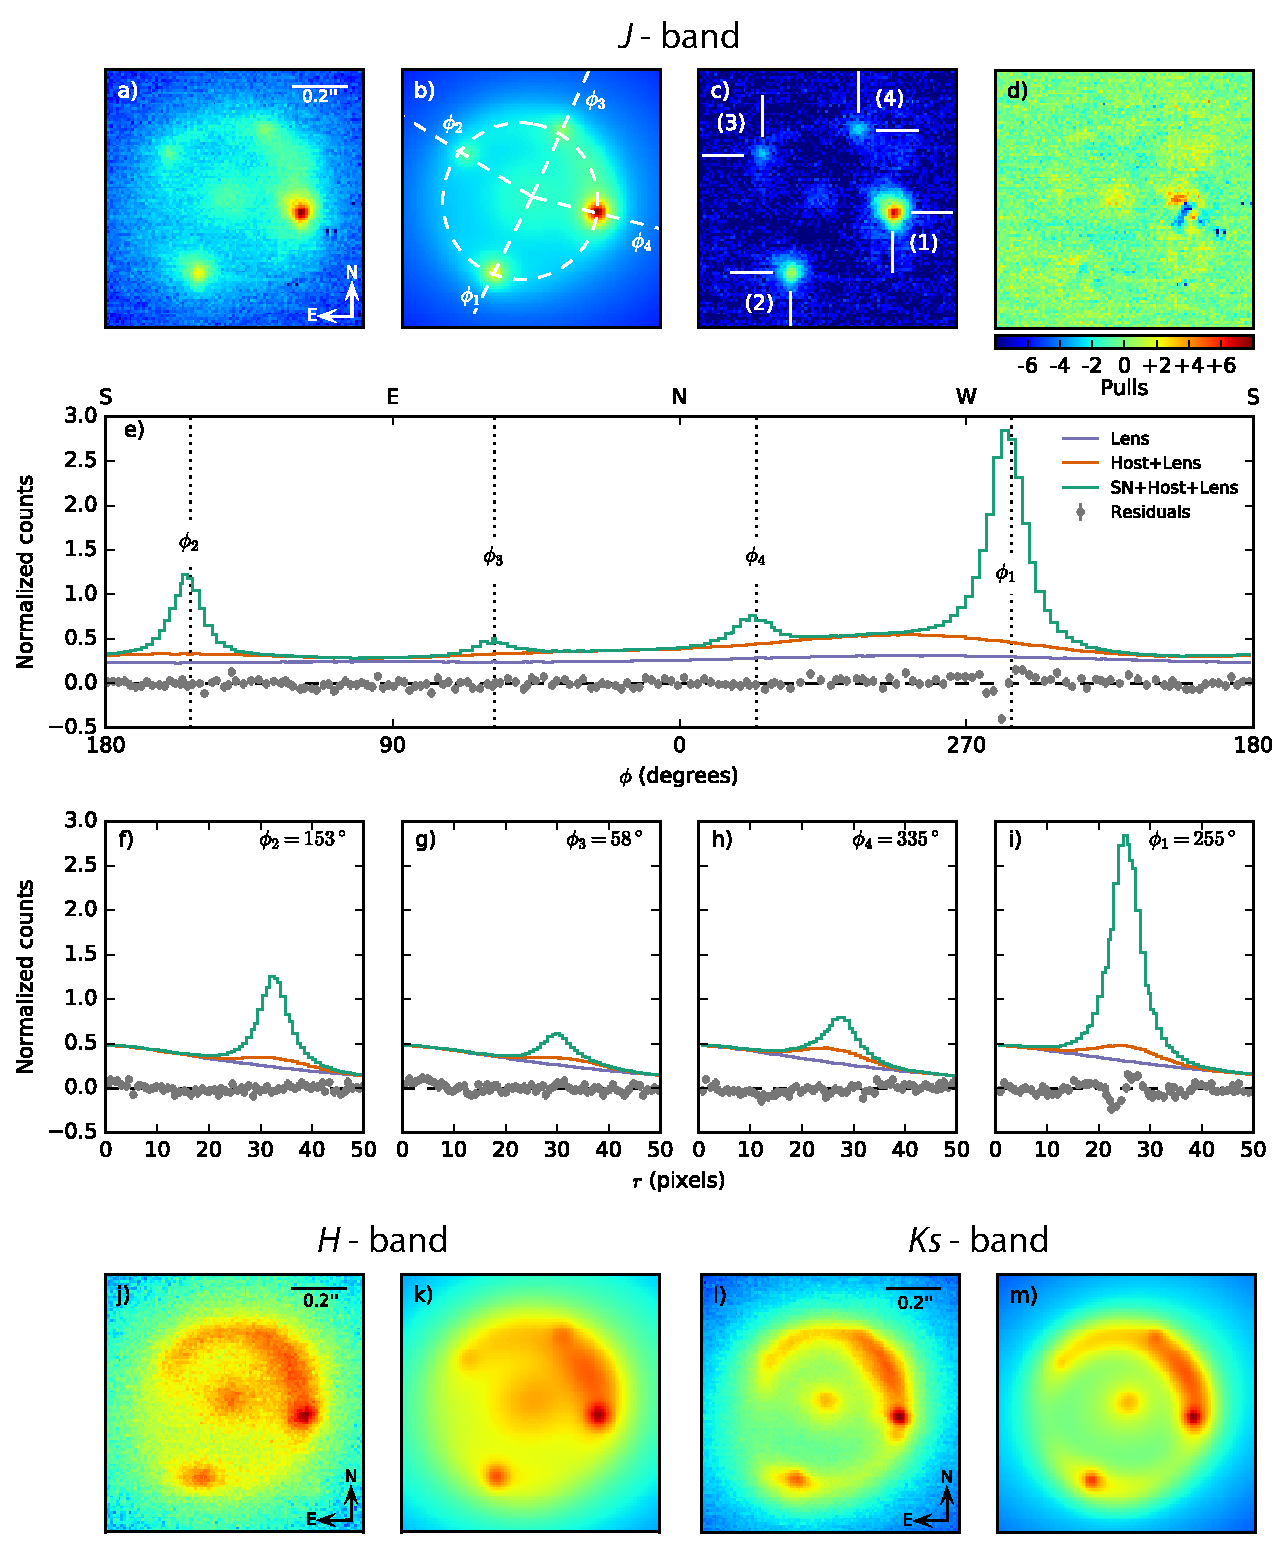
\includegraphics[width=0.95\textwidth]{forward_nirc2_v2.pdf}
	\caption{%
		{\bf a)} NIRC2 \jband image of the \geu system obtained on on Nov 5, 2016. 
		{\bf b)} The model fitted simultaneously to all available epochs as described in the text.  The dashed circle show the 
		position of the host galaxy as described in eq.~\eqref{eq:hostradius}.  The dashed lines are showing the angular 
		positions of the four \sn images. 
		{\bf c)} The subtraction between the data and the host and lens models.  The fitted PSF positions of the four \sn images 
		have been marked.  
		{\bf d)} The ''pulls'', i.e. the residuals normalized with the pixel uncertainties when the lens, host and \sn 
		model is subtracted from the data.  
		{\bf e)} The profile of both the model and the residuals along the host radius marked by the dashed circle in b), The 
		fitted angles, $\phi_i$, of the \sn images are marked by the dotted, black lines.
		{\bf f)} -- {\bf i)}  The radial profiles from the center for the \sn images as marked and labelled in b).
		{\bf j)} -- {\bf k)} NIRC2 \hband image obtained on Oct 23, 2016 and the corresponding fitted model.
		{\bf l)} -- {\bf m} NIRC2 \ksband image obtained on Oct 22, 2016 and the corresponding fitted model.
	\label{fig:nirc2}}
\end{figure*}

%% TABLE: SN image positions
\begin{table}
	\centering
	\caption{%
		The fitted SN positions to the NIRC2 \jband-band images.  The origin is defined as the origin of the \geu system 
		as it is obtained from the model fit and the angle, $0\leq\varphi<2\pi$, is defined from North towards East. All 
		quoted uncertainties are statistical errors obtained from the simultaneous fit described in the text.}
		\label{tb:snpos}
	\begin{tabular}{c r@{\hspace{0.5em}}l r@{\hspace{0.5em}}l}
\hline\hline
Image & \multicolumn{2}{c}{$r$} & \multicolumn{2}{c}{$\varphi$}\\
      & \multicolumn{2}{c}{$('')$} & \multicolumn{2}{c}{(rad)}\\
\hline
1 & 0.251 & (0.001)& 4.468 & (0.002)\\
2 & 0.324 & (0.001)& 2.679 & (0.003)\\
3 & 0.297 & (0.002)& 1.013 & (0.006)\\
4 & 0.276 & (0.001)& 5.860 & (0.005)\\
\hline\hline
\end{tabular}

\end{table}

%% TABLE: Lens model parameters
\begin{table*}
	\centering
	\caption{%
		The fitted lens model parameters as described in eq.~\eqref{eq:lens}.  The origin $(x_0^{(n)},y_0^{(n)})$ of the coordinate
		system are fitted as free parameters for each image $n$.  Angles are defined as $0\leq\theta<2\pi$ from North towards East.
		All quoted uncertainties are statistical fitting errors from each simultaneous fit.
		{\em Note:} Parameters marked with an asterisk ($^{*}$) were fixed to the given value in the fit.}
		\label{tb:lensmodel}
	\begin{tabular}{l | r @{\hspace{0.5em}} l r @{\hspace{0.5em}} l r @{\hspace{0.5em}} l r @{\hspace{0.5em}} l r @{\hspace{0.5em}} l}
\hline\hline
Filter & \multicolumn{2}{c}{$f_S$} & \multicolumn{2}{c}{$r_e$} & \multicolumn{2}{c}{$n_S$} & \multicolumn{2}{c}{$\varepsilon$} & \multicolumn{2}{c}{$\theta$}\\
  & \multicolumn{2}{c}{} & \multicolumn{2}{c}{$('')$} & \multicolumn{2}{c}{ } & \multicolumn{2}{c}{ } & \multicolumn{2}{c}{(rad)}\\
\hline
$K_s$ & 2.43E$-$01 & (1E$-$03) & 0.544 & (0.001) & 0.79 & (0.00) & 0.165 & (0.002) & 0.35 & (0.01)\\
$H$ & 2.08E$-$01 & (2E$-$03) & 0.585 & (0.002) & 0.84 & (0.01) & 0.160 & (0.002) & 0.30 & (0.01)\\
$F160W$ & 1.01E$+$01 & (4E$-$01) & 0.532 & (0.010) & 1.57 & (0.04) & $^*$0.160 &  & $^*$0.30 & \\
$J$ & 1.44E$-$01 & (1E$-$03) & 0.528 & (0.002) & 0.79 & (0.01) & 0.127 & (0.002) & 0.19 & (0.01)\\
$F110W$ & 1.52E$+$01 & (7E$-$01) & 0.529 & (0.013) & 1.66 & (0.05) & $^*$0.127 &  & $^*$0.19 & \\
$F814W$ & 1.45E$-$01 & (9E$-$03) & 0.619 & (0.026) & 1.56 & (0.06) & 0.252 & (0.005) & 0.22 & (0.01)\\
$F625W$ & 1.16E$-$01 & (1E$-$03) & 0.518 & (0.006) & $^*$1.56 &  & $^*$0.252 &  & $^*$0.22 & \\
$F475W$ & 3.69E$-$02 & (2E$-$03) & 0.474 & (0.031) & $^*$1.56 &  & $^*$0.252 &  & $^*$0.22 & \\
$F390W$ & 6.13E$-$03 & (1E$-$03) & 0.588 & (0.147) & $^*$1.56 &  & $^*$0.252 &  & $^*$0.22 & \\
\hline\hline
\end{tabular}

\end{table*}

%% TABLE: Host amplitude and radius parameters
\begin{table*}
	\centering
	\caption{%
		The fitted parameters of the host model, defined in~\eqref{eq:host}.  All quoted uncertainties are statistical 
		fitting errors from each simultaneous fit.}
		\label{tb:hostmodelflux}
	\begin{tabular}{l | r @{\hspace{0.5em}} l r @{\hspace{0.5em}} l r @{\hspace{0.5em}} l r @{\hspace{0.5em}} l r @{\hspace{0.5em}} l}
\hline\hline
Filter & \multicolumn{2}{c}{$a_0$} & \multicolumn{2}{c}{$a_1$} & \multicolumn{2}{c}{$b_1$} & \multicolumn{2}{c}{$a_2$} & \multicolumn{2}{c}{$b_2$}\\
  & \multicolumn{2}{c}{} & \multicolumn{2}{c}{} & \multicolumn{2}{c}{} & \multicolumn{2}{c}{} & \multicolumn{2}{c}{}\\
\hline
$J$ & 2.78E$-$01 & (5E$-$03) & $-$6.93E$-$02 & (2E$-$03) & 4.75E$-$02 & (2E$-$03) & $-$3.43E$-$02 & (1E$-$03) & $-$1.52E$-$02 & (1E$-$03)\\
$H$ & 5.16E$-$01 & (3E$-$03) & $-$1.07E$-$01 & (2E$-$03) & 8.64E$-$02 & (2E$-$03) & $-$4.76E$-$02 & (1E$-$03) & 1.75E$-$03 & (2E$-$03)\\
$K_s$ & 1.47E$+$00 & (1E$-$02) & $-$2.97E$-$01 & (3E$-$03) & 2.56E$-$01 & (3E$-$03) & $-$1.41E$-$01 & (2E$-$03) & 3.53E$-$02 & (2E$-$03)\\
$F625W$ & 3.29E$-$01 & (6E$-$03) & 2.65E$-$02 & (4E$-$03) & 1.04E$-$02 & (3E$-$03) & $-$3.97E$-$02 & (4E$-$03) & $-$1.00E$-$02 & (4E$-$03)\\
$F814W$ & 6.81E$-$01 & (9E$-$03) & $-$5.74E$-$02 & (5E$-$03) & 5.56E$-$02 & (5E$-$03) & $-$8.65E$-$02 & (5E$-$03) & $-$3.44E$-$02 & (5E$-$03)\\
\hline
	\begin{tabular}{l | r @{\hspace{0.5em}} l r @{\hspace{0.5em}} l r @{\hspace{0.5em}} l r @{\hspace{0.5em}} l r @{\hspace{0.5em}} l}
\hline\hline
Filter & \multicolumn{2}{c}{$a_3$} & \multicolumn{2}{c}{$b_3$} & \multicolumn{2}{c}{$c_0$} & \multicolumn{2}{c}{$c_1$} & \multicolumn{2}{c}{$d_1$}\\
  & \multicolumn{2}{c}{} & \multicolumn{2}{c}{} & \multicolumn{2}{c}{$('')$} & \multicolumn{2}{c}{$('')$} & \multicolumn{2}{c}{$('')$}\\
\hline
$K_s$ & 1.76E$-$01 & (2E$-$03) & $-$1.63E$-$01 & (3E$-$03) & 5.831E$-$01 & (3E$-$04) & 3.08E$-$02 & (3E$-$04) & $-$3.54E$-$02 & (3E$-$04)\\
$H$ & 5.72E$-$02 & (2E$-$03) & $-$4.73E$-$02 & (2E$-$03) & 5.787E$-$01 & (8E$-$04) & 3.38E$-$02 & (8E$-$04) & $-$3.11E$-$02 & (8E$-$04)\\
$F160W$ & $-$1.15E$+$00 & (8E$-$01) & $-$1.26E$+$01 & (6E$-$01) & $^*$5.787E$-$01 &  & $^*$3.38E$-$02 &  & $^*$$-$3.11E$-$02 & \\
$J$ & 3.46E$-$02 & (1E$-$03) & $-$2.00E$-$02 & (1E$-$03) & 5.911E$-$01 & (1E$-$03) & 4.49E$-$02 & (1E$-$03) & $-$1.69E$-$02 & (9E$-$04)\\
$F110W$ & $-$4.29E$-$01 & (2E$+$00) & $-$1.54E$+$01 & (1E$+$00) & $^*$5.911E$-$01 &  & $^*$4.49E$-$02 &  & $^*$$-$1.69E$-$02 & \\
$F814W$ & 9.74E$-$02 & (9E$-$03) & $-$1.71E$-$01 & (9E$-$03) & 5.784E$-$01 & (1E$-$03) & 3.51E$-$02 & (8E$-$04) & $-$6.58E$-$03 & (8E$-$04)\\
$F625W$ & 1.74E$-$02 & (9E$-$03) & $-$1.13E$-$01 & (9E$-$03) & 5.788E$-$01 & (2E$-$03) & 3.28E$-$02 & (1E$-$03) & 5.30E$-$03 & (1E$-$03)\\
$F475W$ & $^*$0.00E$+$00 &  & $^*$0.00E$+$00 &  & $^*$5.788E$-$01 &  & $^*$3.28E$-$02 &  & $^*$5.30E$-$03 & \\
\hline\hline
\end{tabular}

\end{table*}

%% TABLE: Host widths
\begin{table}
	\centering
	\caption{%
		The fitted widths, $\sigma_H$, for the host model defined in eq.~\eqref{eq:host}.
	\label{tb:hostmodelwidth}}
	\begin{tabular}{l | r @{\hspace{0.5em}} l}
\hline\hline
Filter & \multicolumn{2}{c}{$\sigma_H$}\\
  & \multicolumn{2}{c}{$('')$}\\
\hline
$K_s$ & 0.080 & (0.001)\\
$H$ & 0.129 & (0.001)\\
$F160W$ & $^*$0.129 & \\
$J$ & 0.102 & (0.003)\\
$F110W$ & $^*$0.102 & \\
$F814W$ & 0.067 & (0.002)\\
$F625W$ & 0.056 & (0.003)\\
$F475W$ & $^*$0.056 & \\
\hline\hline
\end{tabular}
	
\end{table}


As seen in Figure~\ref{fig:nirc2}, the model generally fits the data well.  Four \sn images are clearly visible in the \jband-band 
but from panel~d) we also see that the fit is not perfect.  Discrepancies can mainly be seen for the brightest \sn image, which are 
probably due to an imperfect PSF model, rather than an insufficient background model.  In other words, if the systematic PSF
uncertainties are known, the method can be used to obtain fluxes for the four \sn images.

From the radial profile plots in panels~f)--i) there is an apparent degeneracy between the host model and the \sn profiles given 
that their extrema coincide and have similar width.  However, recall that we only fit one parameter, $\sigma_H$, for the width of 
the host model, as explained in \S\ref{sec:bgmodel}, and the value of this parameter will mainly be determined by the pixels 
between the images located along the dashed circle in panel~b).  Further, by studying the profile along this circle, as shown in 
panel~e), we can conclude that the maximum of the host galaxy amplitude appears to be located between images (1) and (4),  
and the best fit model suggest that the background flux under the \sn images is either increasing or decreasing monotonically.
%This is again reassuring since it means that the pixels surrounding the \sn images can be used to determine the background 
%behind them.

Since we do not expect the image positions to change with neither time nor wavelength, we will fix the positions to the 
values in Table~\ref{tb:snpos} for the remaining of the analysis in this paper.  Using the \jband as the reference, is motivated 
both by the fact that the ratio between the \sn flux and the background is higher than for the other NIRC2 filters, and that we 
have two epochs where the \sn is active.

With the \sn positions fixed we move on to fit the host model for the remaining NIRC2 filters.  The fitted models to the 
\hband- and \ksband-band are shown in panels j)--m) in Figure~\ref{fig:nirc2}.  In the figure, the epochs when the \sn was 
active are shown together with the corresponding data.  The lens and host model parameters are presented in 
Tables~\ref{tb:lensmodel}--\ref{tb:hostmodelwidth}.  


% Similar to the \sn positions we do not expect the position of the host galaxy model, $r_H(\phi)$, to change significantly 
% between different filters.

%% Why is there a difference between the Sersic index for the UVIS and NIRC2?  Is it expected to be wavelength dependent?
%% Close to an exponential profile nS = 1, "which is a good description of spiral galaxy disks and dwarf elliptical galaxies."


\subsection{WFC3 photometry}
The \wfc data were obtained while \geu was active and reference images without \sn light are currently not available.   
However, the photometry of the \sn can still be extracted by using a similar approach as in \S\ref{sec:nirc2}.  

For the data obtained in particular with \wfcuvis we face a similar challenge as for NIRC2, the field of view is too small to
include any isolated stars that could be used to model the PSF.  While conditions in space are relatively stable the PSF 
of \wfc do vary both over the focal plane and in time, and a lot of effort has gone into understanding its characteristics 
\citep{2016wfc..rept...12A,2017arXiv170600386A}.  However, here we use a simple approach that is described in detail 
in \S~\ref{sec:wfcpsf} and only briefly summarised here.  For \wfcuvis we simultaneously fit the parameters of a Moffat profile 
to bright stars observed over time with the same subarray as \geu. The resulting fluxes are then compared to the corresponding 
values obtained from calibrated aperture photometry, following the prescription outlined in \wfc data handbook.  The calculated 
estimated standard deviation, $0.02$--$0.10$~mag, from this comparison is used as the uncertainty of the method, and is 
added to the error budget of the \geu photometry.

The field-of-view for the \wfcir data is larger, and the bright star $20\arcsec$ North of \geu, was included in all observations.
We simultaneously fit a PSF model to all observations of this star, which result in a dispersion $<0.01$~mag with 
respect to the calibrated aperture photometry, if the last epoch is excluded.  Since this epoch does not provide a significant 
contribution to the lightcurve it will also be excluded from the rest of the analysis.

Using one fixed PSF for each filter, we can then follow the procedure from \S\ref{sec:nirc2} and \S\ref{sec:bgmodel}.  Since 
we assume that the PSF is the same for all epochs, we do not convolve the model before comparing with the data in the 
fitting routine, although doing this will result in similar \sn fluxes.  We also omit the host galaxy component from the model for 
the two bluest bands, \hstu and \hstb, since data was not deep enough to detect it at these wavelengths.  For these filters we also 
constrained ourselves to a circular symmetric lens model.

While fitting the combined \geu model works well for \wfcuvis it is significantly more challenging for the \wfcir data.  Both due to the
lower resolution and to the flux ratio between the \sn images and the background being much lower.   The effective radius and the
S\'ersic index for the lens can be constrained by the light beyond the Einstein right, but there is a degeneracy between the different 
components inside the ring.  We therefore decided to only fit a single normalisation parameter for the host model, and fix all other 
parameters to the values obtained for the NIRC2 \jband and \hband-fits, given that effective wavelengths of these bands are similar 
to \hstj and \hsth, respectively.  These may be improved once reference images become available.

Examples of data, model and normalised residual patches are shown in Figure~\ref{fig:wfcforward} for the different \wfc bands, while 
the fitted parameters for the background models are presented in Tables~\ref{tb:lensmodel}--\ref{tb:hostmodelwidth}.  The fitted host
 normalisation parameters are shown in Table~\ref{tb:hostnorm}.  The resulting \sn fluxes from the simultaneous fitting is presented 
in Table~\ref{tb:resolvflux}.

%% Figure with WFC3 patches
%%
\begin{figure*}
	\centering
	\caption{%
		Examples of data, model and residual patches for each \wfc filter.  The residual patches have been normalised by the 
		pixel uncertainty to form the "pull".  For each filter, the epoch where the \sn was the brightest is shown.  This corresponds
		to Oct.~20, 2016 for \hstb, \hstr, and \hsti, Oct.~25, 2016 for \hstu, and Nov.~2nd, 2016 for \hstj and \hsth, respectively.
	\label{fig:wfcforward}}
	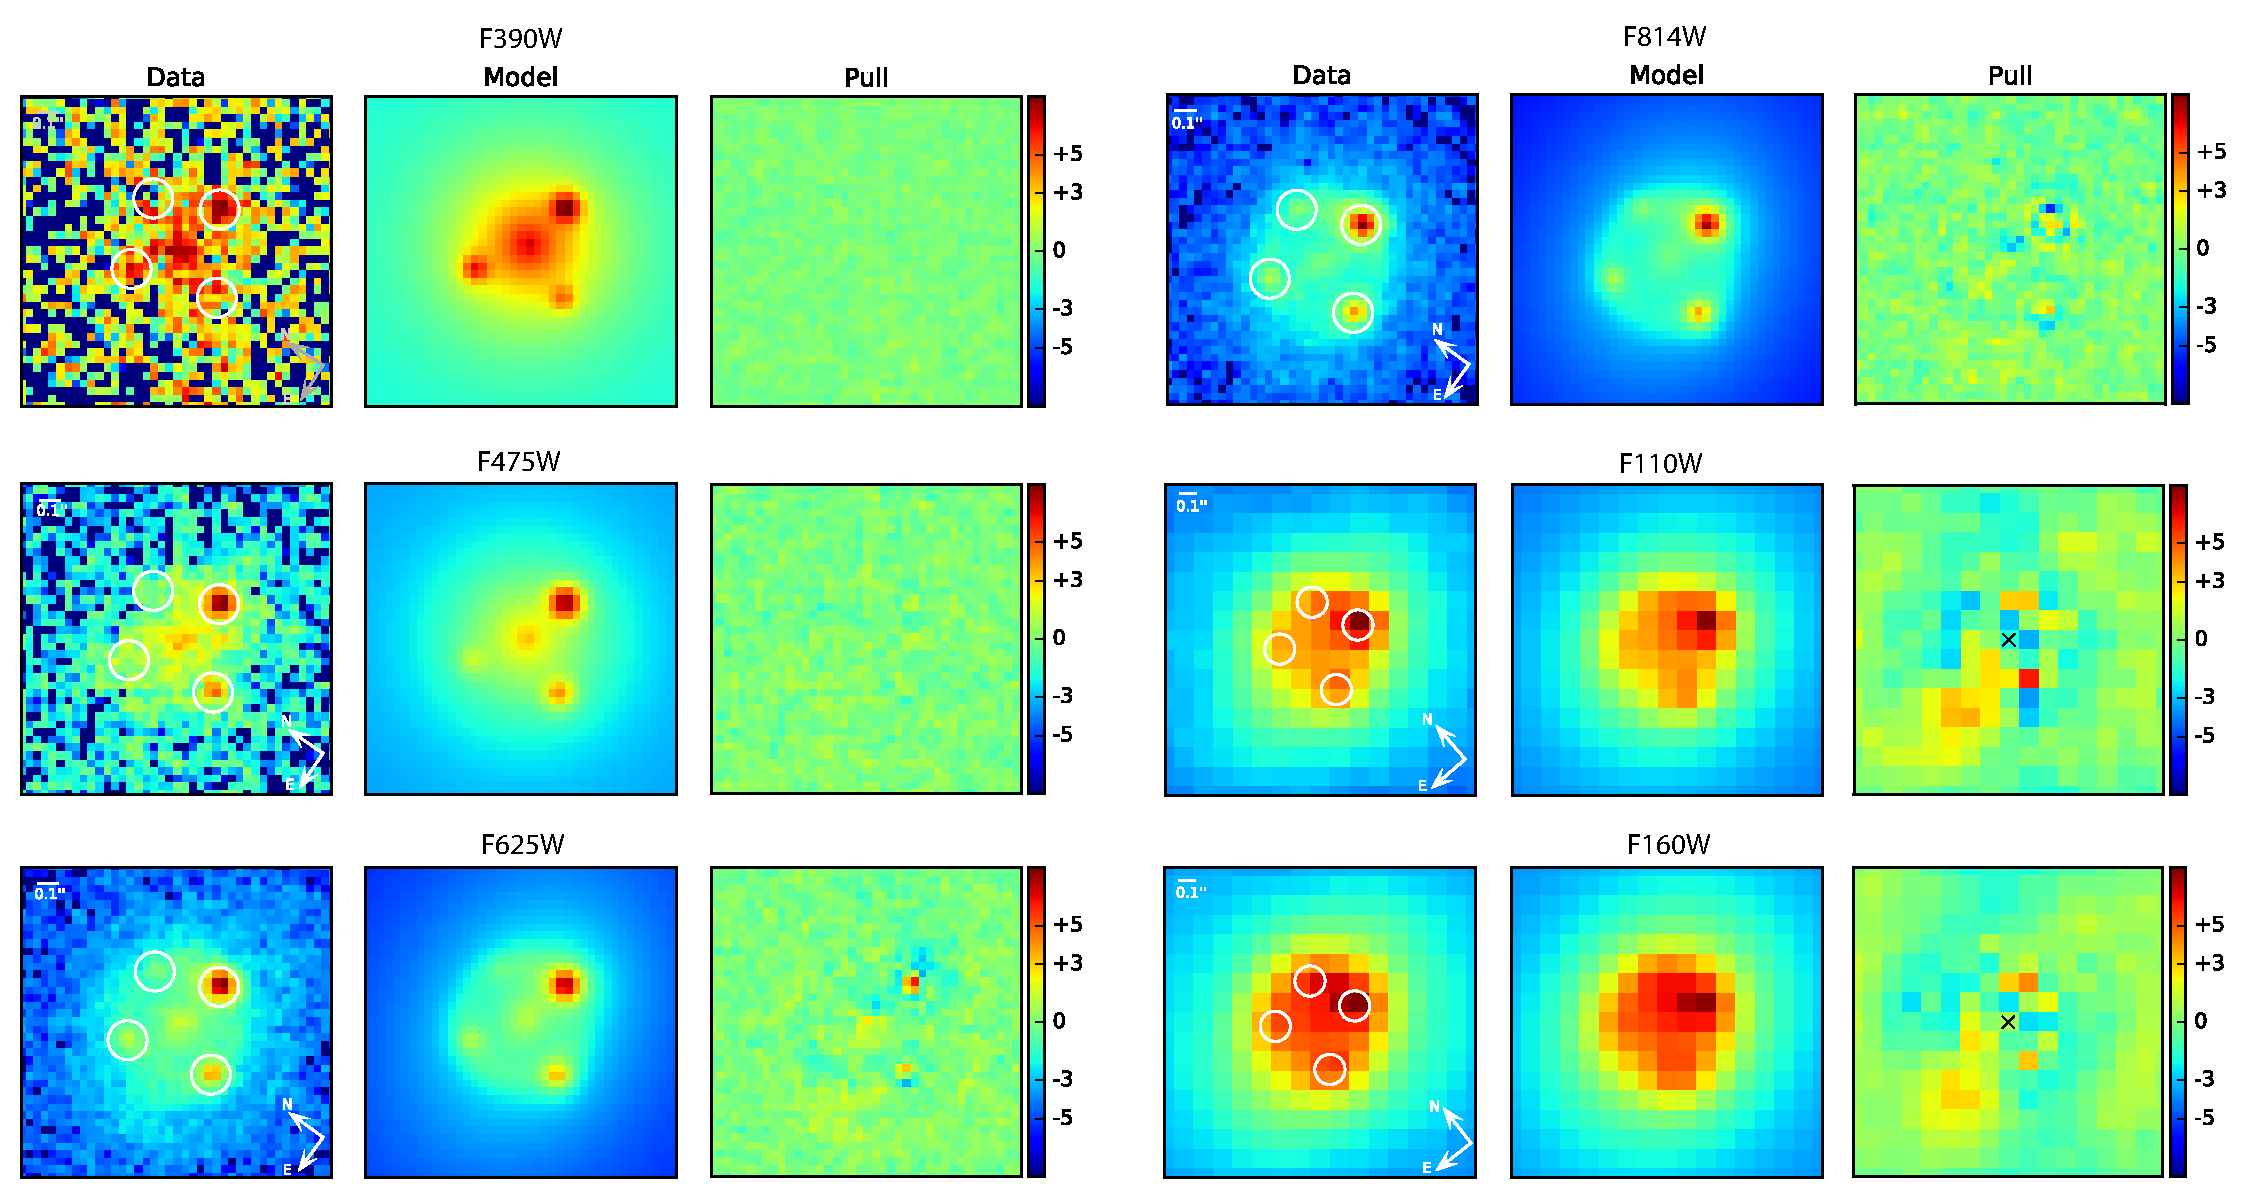
\includegraphics[width=\textwidth]{wfc3_patches.pdf}
\end{figure*}

%% TABLE: Host normalization
\begin{table}
	\centering
	\caption{%
		The fitted normalisation parameter, $h$, for the host model in eq.~\eqref{eq:host} for the \wfcir bands.  In this case
		the parameters $a_i, b_i$ are kept fixed to the values obtained for the NIRC2 $J$ and $H$ bands,
		respectively.
		\label{tb:hostnorm}}
	%\input{host4_model.tex}
    \begin{tabular}{l | r @{\hspace{0.5em}} l}
\hline\hline
Filter & \multicolumn{2}{c}{$\sigma_H$}\\
  & \multicolumn{2}{c}{$('')$}\\
\hline
$K_s$ & 0.080 & (0.001)\\
$H$ & 0.129 & (0.001)\\
$F160W$ & $^*$0.129 & \\
$J$ & 0.102 & (0.003)\\
$F110W$ & $^*$0.102 & \\
$F814W$ & 0.067 & (0.002)\\
$F625W$ & 0.056 & (0.003)\\
$F475W$ & $^*$0.056 & \\
\hline\hline
\end{tabular}

\end{table}

In Table~\ref{tb:resolvflux} we present two different errors for each measurement.  The first error is the statistical fitting error that is obtained 
from the simultaneous fit for each filter.  However, we cannot exclude there are remaining degeneracies between primarily the host model
and the \sn fluxes.  From the residual patches for \hstj and \hsth in Figure~\ref{fig:wfcforward} we can also see that the model we fit
here does not provide very good fit to the data.  In order to estimate the uncertainties from the background model, we rebin  the 
NIRC2 \jband-band data to pixel scales similar the \wfcuvis and \wfcir data.  We then carry out model fits to the data, both using and 
omitting the reference image, and can conclude that the background flux within a FWHM radius under the \sn images varies 
within up to 10\,\% between the two different cases.  For each fitted background model to the \wfc data, we then similarly calculate the
underlying background model flux for each \sn image, and add 10\,\% of this value to the error budget.  This is shown in the second error
column of Table~\ref{tb:resolvflux}.

\subsection{Spectroscopy}
\label{ssec-spectroscopy}
In addition to the spectra presented in \scipap, we analyse the XSHOOTER spectra presented in \citet{2018MNRAS.473.4257C}. They found that \geu can be classified as a high-velocity ($V_{{\rm Si}{\sc ii} \lambda6355}^{\rm max} = 11950 \pm 140$ km s$^{-1}$), high- velocity gradient ($\odot{v} = -110.3 \pm 10.0$ km s$^{-1}$) and “core-normal” SN Ia. The strength of various features (measured though their pseudo-equivalent widths) argue against SN \geu being a faint, broad- lined, cool or shallow-silicon SN Ia.

The spectra also reveal narrow absorption and emission lines, marked by the dashed vertical lines, from which the redshifts of the lens ($z = 0.2166 \pm 0.0001$, blue lines) and SN host galaxy ($z = 0.4090 \pm 0.0001$, red lines) were determined. Zoomed in view in rest-frame wavelengths of the Ca~{\sc ii} H~\&~K and Na~{\sc i}~D absorption features are shown in Fig.\ref{fig:spec_panels}, together with the $H_{\alpha}$, [N {\sc ii}] and O~{sc ii} emission lines. The $H_{\alpha}$ and [N {\sc ii}] emission lines at z = 0.2166 were used to fit the velocity dispersion of matter in the lensing galaxy, $\sigma_v = 163^{+41}_{-27}$ km/s (old number from \scipap).

For the lensing galaxy, we measure the equivalent widths (EW) of the Ca~{\sc ii} H~\&~K and Na~{\sc i}~D absorption features to be 9.93 \AA \, and 2.12 \AA \,, respectively. At the host galaxy redshift, we measure EWs of 2.25 \AA \, and 3.60 \AA \, for the Ca~{\sc ii} H~\&~K and Na~{\sc i}~D absorption features, respectively.

Using the relations from Barbon (1990), Turato et al. (2003) and Poznanski et al. (2011) that relate the Na~{\sc i}~D EW and color excess, $E(B-V)$, we find that $E(B-V)_{\rm lens} \sim 0.83 \pm 0.5$ mag and $E(B-V)_{\rm host} \sim 1.47 \pm 0.5$ mag. (It should be noted that these relations are only "well defined" for EW < 1.0 \AA \, and that the "theoretical" relation is between EW and optical depth, $\tau \sim A_V$, and that $A_V = R_V \times E(B-V)$ with $R_V$ =3.1 is usually assumed?). 

To reduce the degeneracy between $E(B-V)_{\rm host}$ and $E(B-V)_{\rm lens}$ when fitting the light curves, we introduce a prior based on the ratio of the Na~{\sc i}~D absorption in the host and lens, such that $E(B-V)_{\rm host} = f \times E(B-V)_{\rm lens}$, with $1.6 \leq f \leq 1.8$.
%Lens:
%Poznanski, 2012 EBV= 4.2465252214
%Poznanski, 2011 EBV= 0.830730337068
%Turatto, 2003, EBV= 0.32887640449 1.04016853931
%Barbon, 1990 EBV= 0.529494382016
%Host:
%Poznanski, 2012 EBV= 232.450124618
%Poznanski, 2011 EBV= 1.4695912879
%Turato, 2003, EBV= 0.566592107125 1.79788734146
%Barbon, 1990 EBV= 0.900925167382

% Other analyses to do?
% put stuff on BPT diagram?
% far fetched host galaxy redshift(s)?

\begin{figure*}
	\centering
	\caption{Zoomed in panels on narrow absorption and emission lines in the XSHOOTER spectrum
	\label{fig:spec_panels}}
	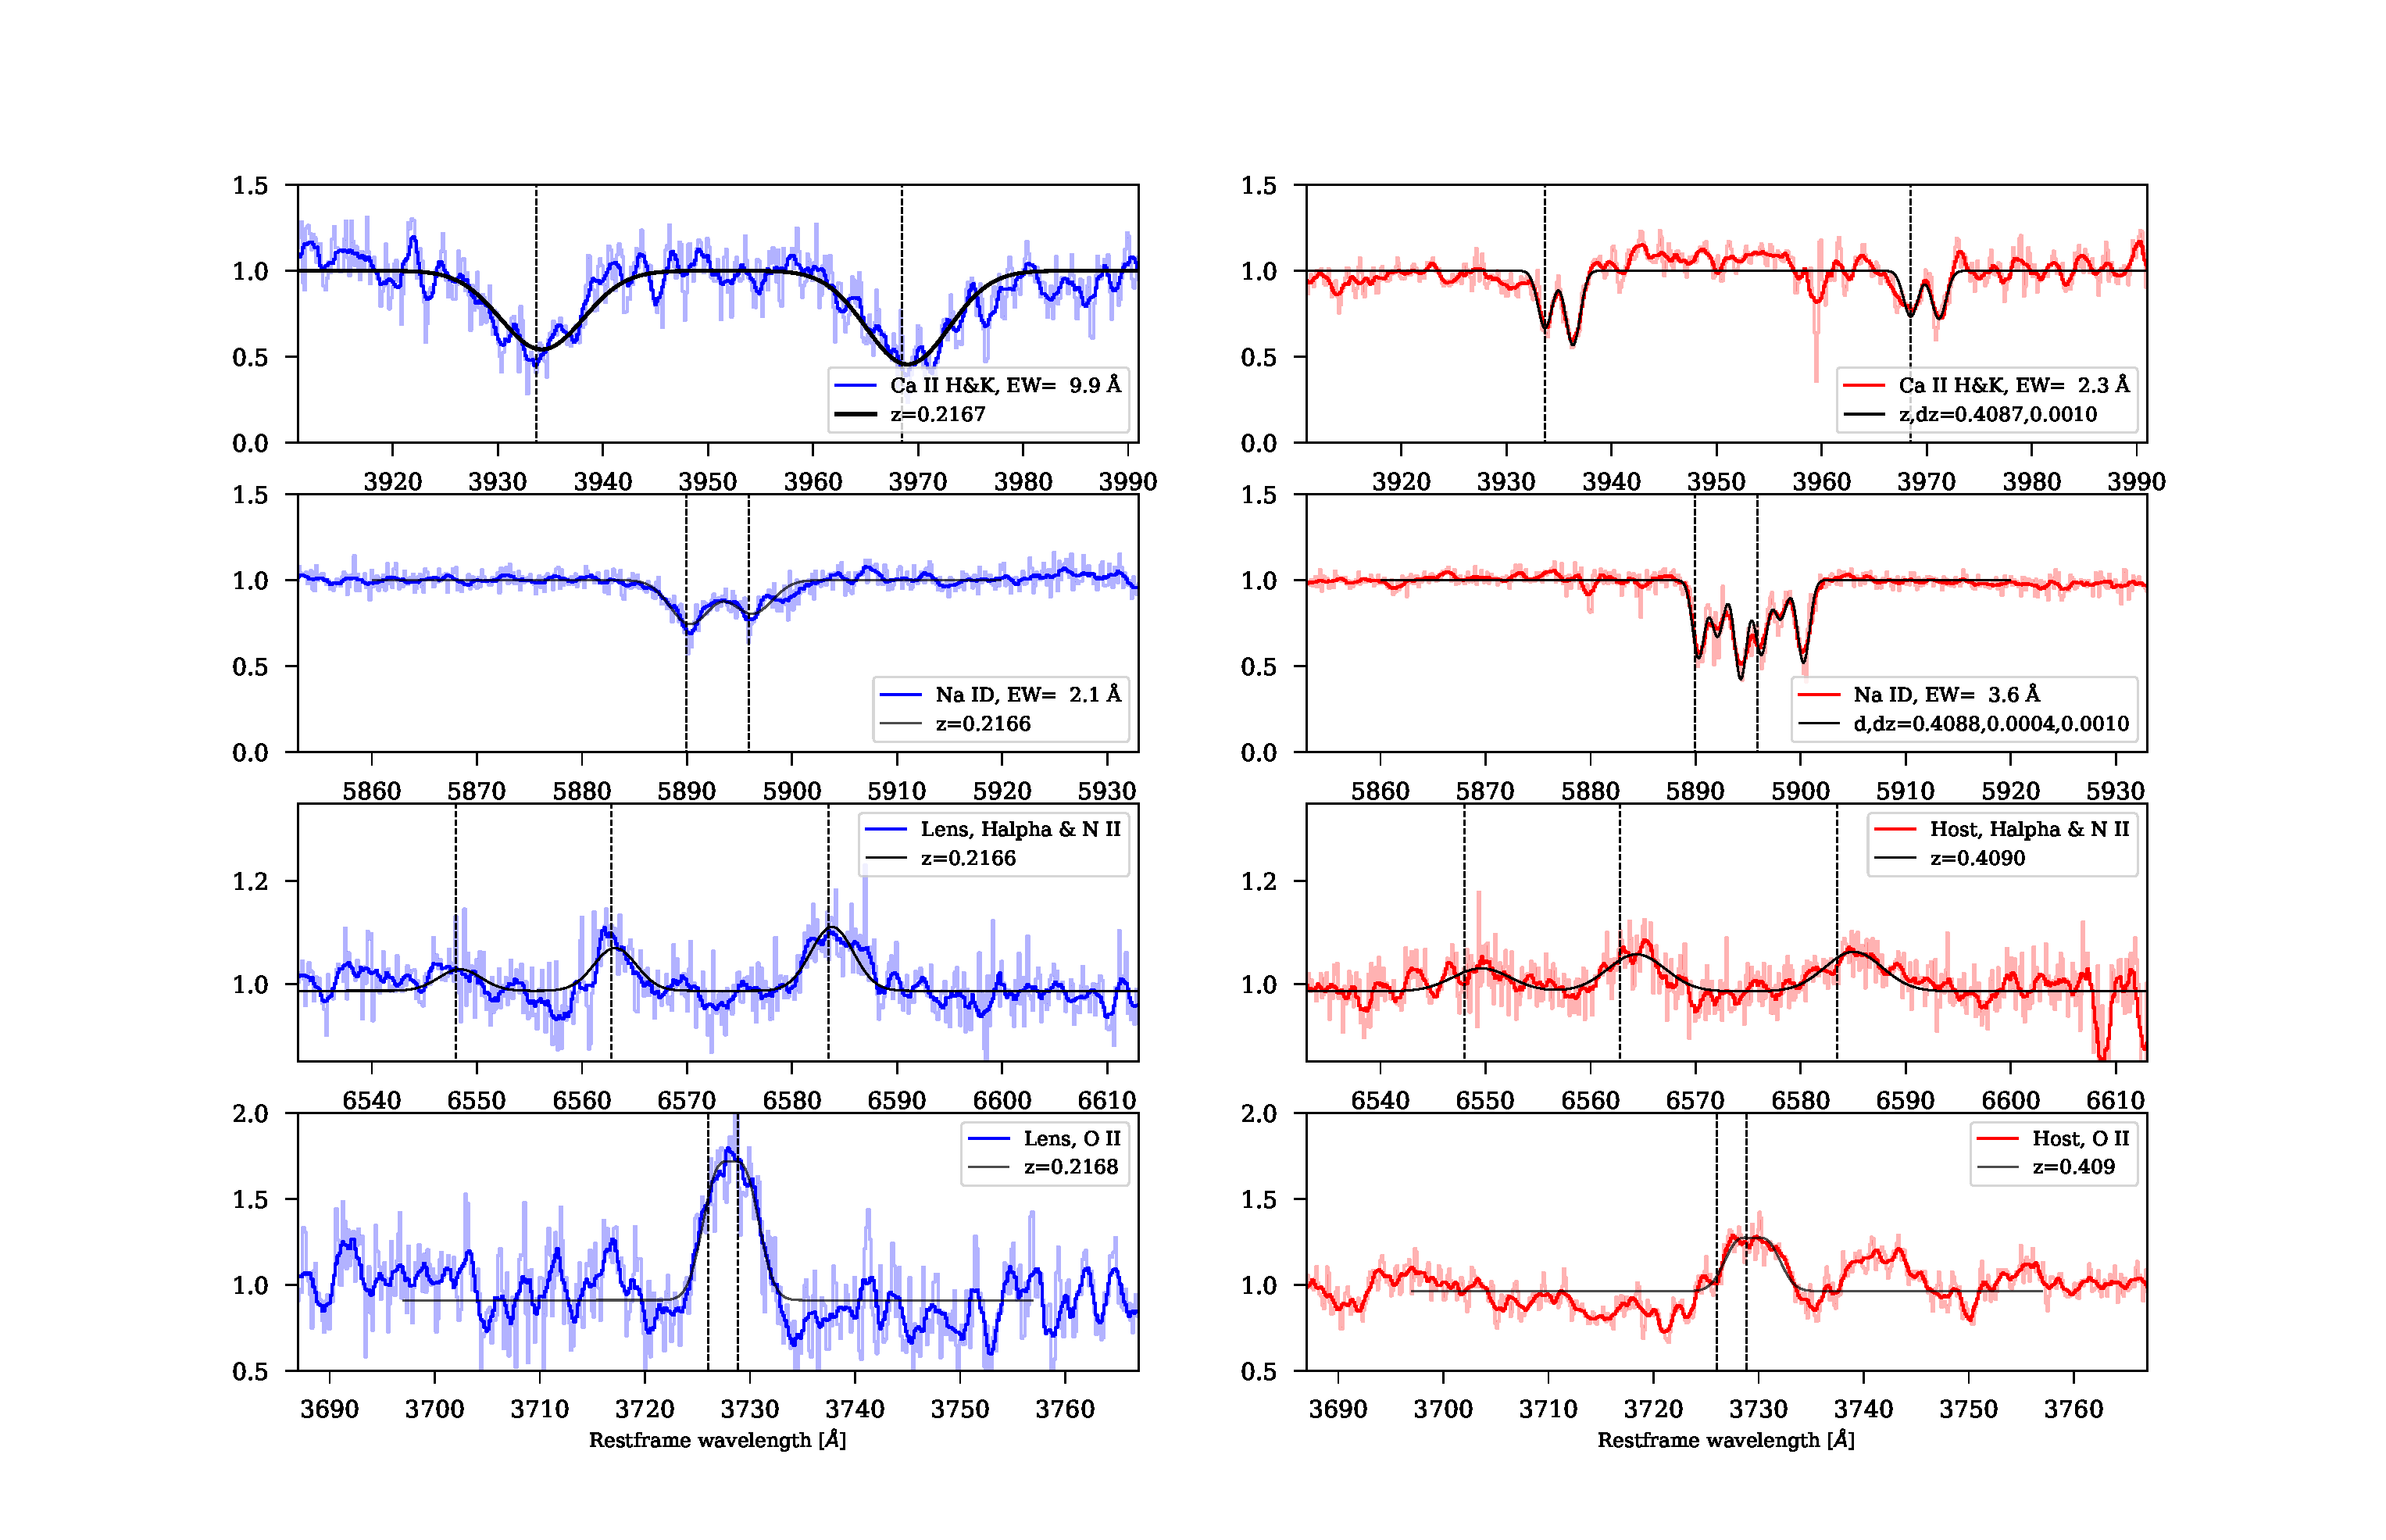
\includegraphics[width=\textwidth]{spec_panels.pdf}
\end{figure*}

% There are also additional spectra:
%2016-10-09 NTT+EFOSC (PESSTO)
%2016-10-09 FTN+FLOYDS
%2016-10-10 NTT+EFOSC (PESSTO)
%2016-10-15 GTC-OSIRIS (Cano+2017)
%2016-10-18 GTC-OSIRIS (Cano+2017)
%2016-10-22 DCT+LMI (Cenko?)
%2016-10-26 P200+DBSP
%2016-10-26 Keck2+DEIMOS (Filippenko)
%2016-10-30 GTC-OSIRIS (Cano+2017)
%2016-10-31 Keck1+LRIS (Lunnan - what happened to this data?)
%2016-11-02 Keck1+LRIS (Kulkarni)
%2016-11-18 GTC-OSIRIS (Cano+2017)
%2016-11-28 Keck1+LRIS (Kulkarni)
%2016-11-30 GTC-OSIRIS (Cano+2017)
%2016-12-15 GTC-OSIRIS (Cano+2017)
\subsection{Constructing the SN model}
\sd{I just wrote a section here to describe the model before writing the results of the fits in Section~\ref{sec:results}}
Here, we describe the SN model constructed to derive the time-delay, magnification and extinction parameters for iPTF16geu. We construct a multiple-image model for an SN~Ia using \texttt{sncosmo} with a \texttt{Hsiao} model \citep{2007ApJ...663.1187H}, which incorporates a large spectral library for a diverse range of SNe~Ia. 
  We fit the model to the observations using a $\chi^2$ likelihood with two terms for the ground based and the HST data. For the ground based data we compare the sum of the models to the observations, whereas for the HST data we compare the individual images. 
\begin{equation}
\label{eq:chi}
\begin{aligned}
\chi ^2 &= \left(\sum_{\lambda}^{\mathrm{Ground}}\frac{\left[\left(\sum_i^{N} F_i^{model}(t,\lambda)\right)-F^{data}(t,\lambda)\right]^2}{\sigma^2(t,\lambda)}\right)+ \\
&\quad \left(\sum_{\lambda}^{\mathrm{HST}}\sum_i^{N}\frac{\left[F_i^{model}(t,\lambda)-F_i^{data}(t,\lambda)\right]^2}{\sigma_i^2(t,\lambda)}\right),
\end{aligned}
\end{equation}
where $F$ is the flux, $t$ is the epoch of the SN~Ia light curve, $N$ is the number of images and $\lambda$ is the effective wavelength of each filter. 

For each of the four individual images, we apply an extinction correction for the host and lens galaxies as well as the Milky Way. We assume a standard MW reddening law \citep{1989ApJ...345..245C} for the MW, lens and host galaxies. For the MW, we set the slope of the reddening law, R$_V$ to 3.1, however, for the host and lens galaxies, we fix  R$_V$ to 2. This is using the slope of the luminosity-colour relation from the most updated compilations of cosmological samples \citep[see;][]{2018ApJ...859..101S,2018arXiv181102374D} which can be applied to iPTF16geu, since it shows distinct features of core-normal SNe~Ia \citep[e.g.,][]{2006PASP..118..560B}, used for cosmological constraints. Therefore, in our model fit, we include the following parameters 
\begin{itemize}
    \item The stretch, s, for the SN
    \item The colour excess, $E(B-V)$ in the host galaxy
    \item The colour excess, $E(B-V)$ for the individual images in the lens galaxy 
    \item The time of maximum $t_{0}$ for each of the four images, and hence, the time-delays between the images
    \item The magnification for each of the four images
\end{itemize}


From the spectroscopic analysis described in Section~\ref{ssec-spectroscopy}
we use a prior on the relation between the $E(B-V)_{\rm host}$  and $E(B-V)_{\rm lens, 1}$ \sd{I am not sure why this is only for Image 1, is the spectrum only for Image 1?}. We fit this model to the data using a nested sampling software, \texttt{nestle} implemented in \texttt{sncosmo}. 

\begin{figure*}
    \centering
    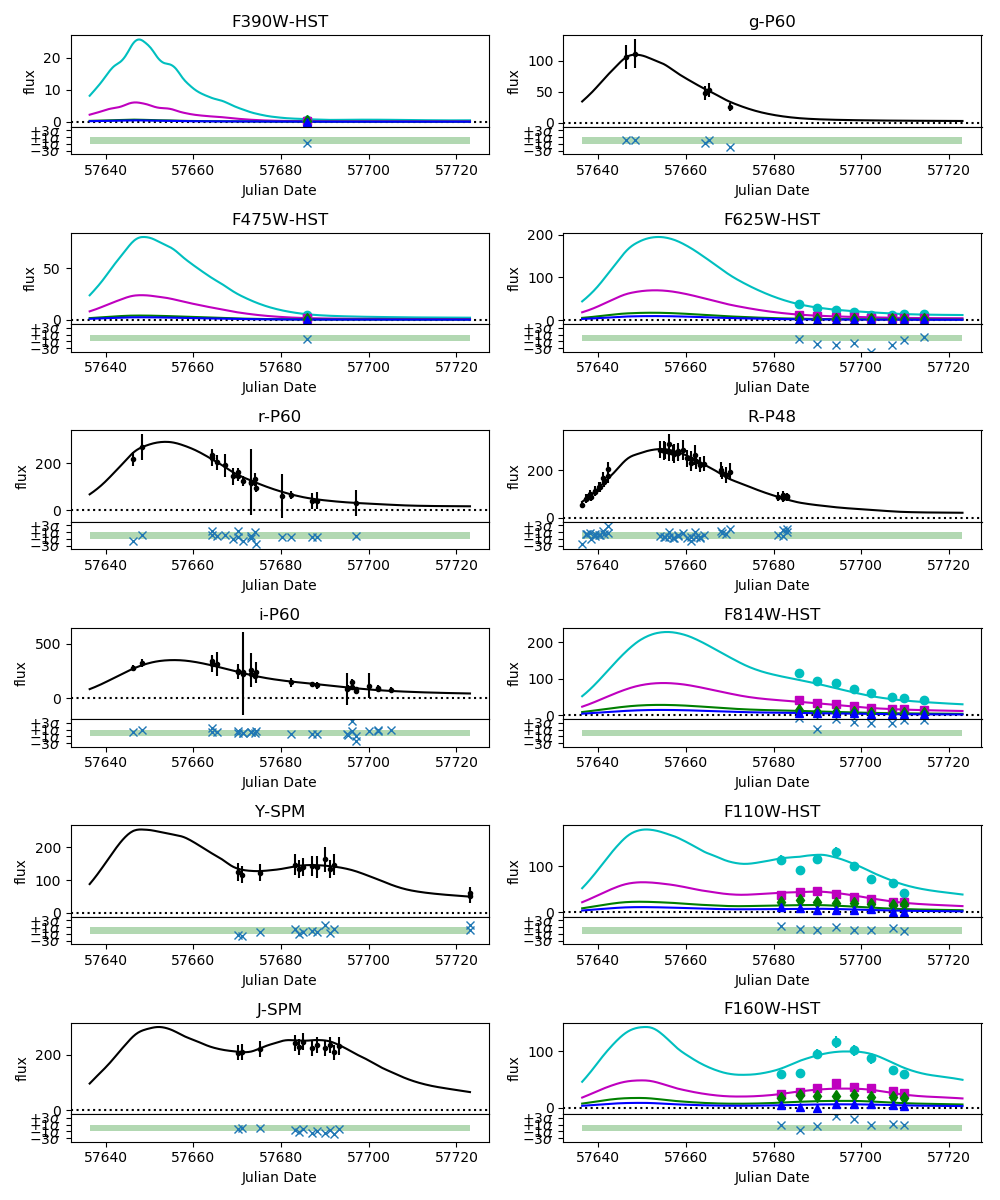
\includegraphics[width=.9\textwidth]{16geu_lcfit.png}
    \caption{Model fit to the photometry for iPTF16geu (see text for details). The ground based data are plotted in black whereas the HST data for Image 1 is in cyan, Image 2 in magenta, Image 3 in green and Image 4 in blue. The residuals from the best fit are shown in the panel under each filter. The filters are plotted in ascending order of effective wavelength.}
    \label{fig:16geu_lc}
\end{figure*}

\section{Results}
\label{sec:results}
In this section, we present the results of fitting the multiple-image SN model to the observations of iPTF16geu. For our analyses, we add an error term to the diagonal elements of the covariance matrix corresponding to 5$\%$ of the flux. This term represents systematic errors relating to unaccounted for effects, e.g. microlensing. We derive this term by requiring the reduced $\chi^2$ of the fit to be $\sim$ 1. 
 We present the resulting values of the time-delays between the images (Section~\ref{ssec-time_delay}) and the properties of the extinction due to dust in the host and lens galaxies (Section~\ref{ssec-extinction}). 




\begin{table*}
\centering
\begin{tabular}{|c|c|c|c|c|}
\hline
Parameter & Image 1 & Image 2 &  Image 3 & Image 4 \\
\hline\hline
t$_{max}$ &  57653.25 ($\pm$ 0.008) & -0.713 ($\pm$  0.848) & -1.4.08  ($\pm$ 1.03) & -0.637 ($\pm$ 1.344) \\
Magnification & -3.919 ($\pm$ 0.266) & 2.84 ($\pm$ 0.271) &  2.109 ($\pm$ 0.287) & 1.519 ($\pm$ 0.299) 
\\
lens E(B-V) &  0.166 ($\pm$ 0.0189) &  0.157 ($\sim$ 0.08) & 0.679 ($\pm$ 0.131) & 0.794 ($\pm$ 0.142) \\
\hline
\end{tabular}
\label{tab:params}
\end{table*}



\subsection{Time-delays}
\label{ssec-time_delay}
We fit the time of maximum for the four images and calculate the time-delay for images 2,3,4 relative to Image 1  t$_{01}$, t$_{02}$, t$_{03}$, t$_{04}$. The summary of the parameter values is presented in Table~\ref{tab:params}. 

\subsection{Differential extinction}
\label{ssec-extinction}
In this section, we determine the parameters for the extinction in the different images. The resulting parameters from the fit are summarised in Table~\ref{tab:params}. We find a moderate amount of extinction in Images 1 and 2 (0.166 and 0.208 respectively), however, Images 3 and 4 have significantly larger extinction (0.653 and 0.794 respectively). The total amplification for iPTF16geu from this fit is 61.7 $\pm$ 18.4.

\begin{figure}
    \centering
    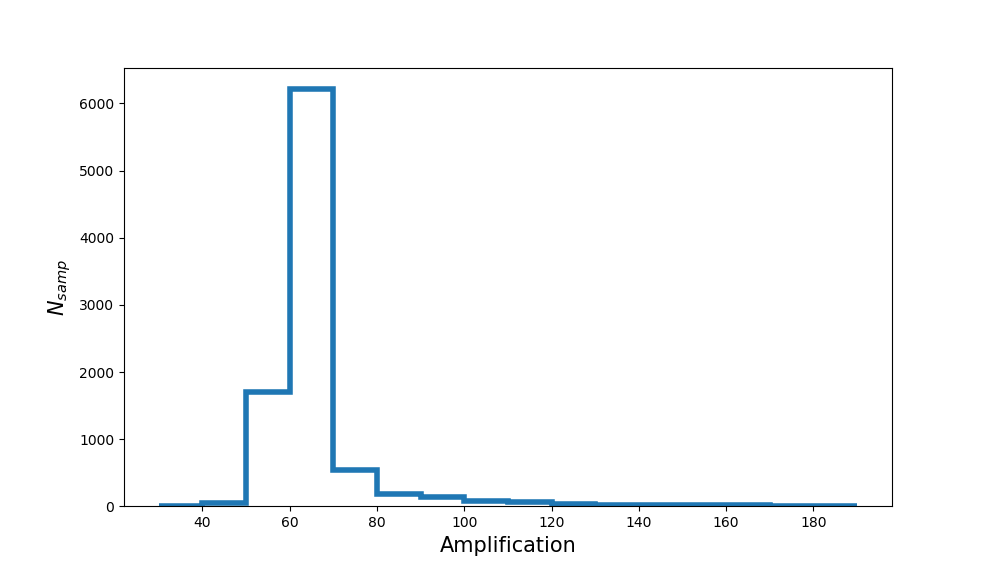
\includegraphics[width=.5\textwidth]{amplification_Rv2.png}
    \caption{The posterior distribution for the total amplification fitting the multiple-image \texttt{sncosmo} model described in the text. The median value is 62.3 with a 68$\%$ credible region between (58.7, 66.81).}
    \label{fig:amp}
\end{figure}

We test the impact of changing the input R$_V$ for the lens and host galaxies. For a lower R$_V$ of 1.5, we obtain a higher $E(B-V)$ of 0.80$\pm$ 0.18 for Image 3, and a smaller total amplification of 54.6 $\pm$ 21.2, which is consistent with the value for the fiducial case. Conversely, for higher R$_V$ values of 3.1, the inferred $E(B-V)$ for Images 3 and 4 are 0.57($\pm$ 0.059) and 0.695 ($\pm$ 0.143) and the amplification is 75.1 $\pm$ 20.6. The total amplification distribution is plotted in Figure~\ref{fig:amp}. 

%Figures and tables should be placed at logical positions in the text. Don't
%worry about the exact layout, which will be handled by the publishers.
%
%Figures are referred to as e.g. Fig.~\ref{fig:example_figure}, and tables as
%e.g. Table~\ref{tab:example_table}.

% Example figure
%\begin{figure}
%	To include a figure from a file named example.*
%	Allowable file formats are eps or ps if compiling using latex
%	or pdf, png, jpg if compiling using pdflatex
%	\includegraphics[width=\columnwidth]{example}
%   \caption{This is an example figure. Captions appear below each figure.
%	Give enough detail for the reader to understand what they're looking at,
%	but leave detailed discussion to the main body of the text.}
%   \label{fig:example_figure}
%\end{figure}



\section{Conclusions}

%The last numbered section should briefly summarise what has been done, and describe
%the final conclusions which the authors draw from their work.

\section*{Acknowledgements}

%The Acknowledgements section is not numbered. Here you can thank helpful
%colleagues, acknowledge funding agencies, telescopes and facilities used etc.
%Try to keep it short.

%%%%%%%%%%%%%%%%%%%%%%%%%%%%%%%%%%%%%%%%%%%%%%%%%%

%%%%%%%%%%%%%%%%%%%% REFERENCES %%%%%%%%%%%%%%%%%%

% The best way to enter references is to use BibTeX:

\bibliographystyle{mnras}
\bibliography{geu} % if your bibtex file is called example.bib

%%%%%%%%%%%%%%%%%%%%%%%%%%%%%%%%%%%%%%%%%%%%%%%%%%

%%%%%%%%%%%%%%%%% APPENDICES %%%%%%%%%%%%%%%%%%%%%

\appendix
\section{Forward modelling of the \geu images}
\label{sec:bgmodel}
A model,  $F(r,\phi)$, of the observed 2D shape of the \geu system in a broadband image, can be expressed as a 
combination of parametric lens and host models, $L(r,\phi)$ and $H(r,\phi)$, and the point spread function (PSF) of the 
image as
\begin{eqnarray*}
	F(r,\phi) & = & A_n\cdot PSF\otimes \left[L(r,\phi) + H(r,\phi)\right] +\\
	& + & \sum\limits_{i=1}^{4}\left( f_{i}^{(n)} PSF(r_i,\phi_i) \right)+ B_n
\end{eqnarray*}
where the coordinates $(r,\phi)$ are defined with respect to the center (which are treated as nuisance parameters in the fit)
of the system in each image $n$, and the angle $0 \leq \phi < 2\pi$ runs from North towards East.  The index, $i=1,2,3,4$ runs 
over the four SN images, and $n$ runs over all observed epochs for a given band.  Further, $f_{i}^{(n)}$ and $(r_i,\phi_i)$ are 
the fluxes and coordinates of the SN images.  The amplitude, $A_n$, can be used to account for varying photometric 
calibration, but must be kept fixed for at least one image in each band in order to break the degeneracy between the  
parameters for $L$ and $H$.  We also allow for the background, $B_n$ to vary between images. 

The lens, $L$, is modelled by a S\'ersic profile \citep{1963BAAA....6...41S}
\begin{equation}
	L(r,\phi) = S^{n_S}(r,\phi) = f_S\cdot \exp\left\{-b_n\left[\left(\frac{r_S(\theta,\epsilon;\phi)}{r_e}\right)^\frac{1}{2n_S} - 1\right]\right\}\,
	\label{eq:lens}
\end{equation}
where $r_S(\theta,\epsilon;\phi)$, is generalized to allow for an elliptical model with ellipticity, $\epsilon$, and rotation, $\theta$.  Here,
$b_n$ (solved for numerically) is defined such that $r_e$ contains half of the total luminosity , $f_S$ is the intensity, and $n_S$ is
the S\'ersic index.  
%In the cases where this model is not sufficient for describing the nucleus of the lensing galaxy we also add an 
%exponential, $S^1(r,\phi)$, with an effective radius, $r_\mathrm{exp}$, but with the same ellipticity and orientation 
%as for $S^{n_S}(r,\phi)$.

The host galaxy is expressed as a Gaussian profile according to
\begin{equation}
	H(x,y) = h\cdot f_H(\phi)\cdot\exp\left\{-\frac{(r - r_H(\phi))^2}{2\sigma_H^2}\right\}\, ,\label{eq:host}
\end{equation}
where  the amplitude, $f_H(\phi)$ and radius, $r_H(\phi)$ are defined as
\begin{eqnarray}
f_H(\phi) & = & \frac{a_0}{2} + \sum\limits_{j=1}^3 a_j\cdot\sin(j\phi) + b_j\cdot\cos(j\phi)\, ,\label{eq:hostflux} \\ 
r_H(\phi) & = & \frac{c_0}{2} +  c_1\cdot\sin(\phi) + d_1\cdot\cos(\phi)\, .\label{eq:hostradius}
% \sigma_H(\phi) & = & \frac{g_0}{2} + \sum\limits_{j=1}^3 g_j\cdot\sin(j\phi) + h_j\cdot\cos(j\phi)\, .
\end{eqnarray}
The parameter $h$, and the parameters $a_0, a_j, b_j$ cannot be fitted simultaneously.  The former is only allowed as a free parameter
for \wfcir when $a_0, a_j, b_j$ is fixed to the solution for the LGS-AO data.

We also allow for a rotation, $\delta_n$ of the full system, i.e. $\phi \rightarrow \phi + \delta_n$ between images.  These parameters 
must be fixed for at least one image to break the degeneracy with the angle dependent model parameters.

In its most general implementation the number of free parameters of the model can be:
\begin{itemize}
\item $2\times n + (n-1)$ for the position and rotation in each image
\item $4\times 3 \times n$ for the SN fluxes and positions
\item $n-1$ for the normalization of the model in each image
\item $5$ for the lens model
\item $11$ for the host model
\end{itemize}
which results in a total of $14 + 16n$ parameters.  However, when fitting this model to the data we will generally require 
that the SN positions are the same between different filters.  
%In practice, we also applied an iterative approach where the complexity of the model was increased in each step and the Bayesian 
%Information Criterion \citep[BIC,][]{schwarz1978} was calculated.  The more complex model was only kept if  $\Delta\mathrm{BIC}>10$.


%% WFC3 PSF model
%%
\section{Empirical point-spread function model for \wfc}
\label{sec:wfcpsf}
Although the shape and variability of the point-spread-function (PSF) of \wfc has been studied in great detail 
\citep{2016wfc..rept...12A,2017arXiv170600386A}, a simple time-independent PSF model will be used here.  
We fit the profile,
\[
	PSF(x,y;A,\alpha,\gamma) = A\cdot \frac{\alpha - 1}{\pi\gamma^2}\left[1 + \left(\frac{x^2 + y^2}{\gamma^2}\right)\right]^{-\alpha}\,,
\]
as described by \citet{1969A&A.....3..455M},  where, $x$ and $y$ are pixel coordinates and $A$, $\alpha$ and $\gamma$ are 
free parameters.  The profile is fitted to bright isolated stars observed between 2010 and 2017 and with the same subarray, 
\uvisaperture, used for the \geu.  The data are also drizzled to the same resolution, and with the same kernel as for our science 
observations.  

The \wfcir observations of \geu was obtained with a larger field-of-view than \wfcuvis as shown in Fig.~\ref{fig:psfnir}, and 
included a bright, but unsaturated, star $\sim20\arcsec$ North of the object.  The star was visible in all \wfcir and bands and
could be used to determine the PSF shape for these filters using the same approach as for \wfcuvis. 
%% For the WFC3/IR observations of iPTF16geu we offset the pointing with about 20" (160 pixels) from the center to avoid having
%% the nearby bright star to fall on the detector.  On the other hand the, for the observations of standard stars used for 
%% deriving the PSF the pointing was never chosen to that the star fell in the center. All standard star observations were obtained using
%% smaller 256x256 subarray.

The PSF fit is carried out to all data in a given filter.  While the amplitude, $A$, is fitted to each exposure, the parameters, 
$\alpha$ and $\gamma$, are only allowed to vary between different filters.   The fitted amplitudes of each star are then compared to the 
corresponding value obtained from aperture photometry.  For the latter we follow the guidelines in the \wfc data handbook 
\citep{wfc3handbook} and always use a fixed aperture radius of $0.4\arcsec$, for which zero points have been derived.  
The two sets of values are used both to calculate the aperture correction for the PSF photometry and to assess the quality of this simple 
time-independent PSF model.  The later is quantified by the estimated standard deviation between the PSF and and aperture
photometry for all observations in a given filter.  These values are then added in quadrature to the photometry error budget.

The fitted parameters and the $\sigma$ values are given in Table~\ref{tb:psf} for the different filters.  For the \wfcir data the last 
epoch from Nov 22, 2016 was excluded from the fits since this was found to deviate significantly from the others.
% and a  couple of examples of profile fits are shown in Fig.~\ref{fig:psf}.

\begin{table}
\centering
\caption{%
   Table of the derived PSF parameters and the estimated standard deviations PSF and aperture photometry 
   for all stars in each given.  Here, the full width at half maximum was calculated as 
   $\mathrm{FWHM} = 2\gamma\left(2^{1/\alpha}-1\right)^{1/2}$. See the text for further details.
  \label{tb:psf}
}
\begin{tabular}{ccccc}
\hline\hline
Band & $\alpha$ & $\gamma$ & FWHM & $\sigma$ \\
  & & (pix) & (pix) & (mag)\\
\hline
F390W & 3.245 & 2.398 & 2.340 & 0.072 \\
F475W & 3.114 & 2.531 & 2.528 & 0.096 \\
F625W & 1.844 & 1.592 & 2.151 & 0.083 \\
F814W & 1.798 & 1.414 & 1.939 & 0.024 \\
F110W & 2.929 & 1.343 & 1.388 & 0.007 \\
F160W & 2.646 & 1.327 & 1.452 & 0.006 \\
\hline\hline
\end{tabular}

\end{table}

%\begin{figure*}
%\centering
%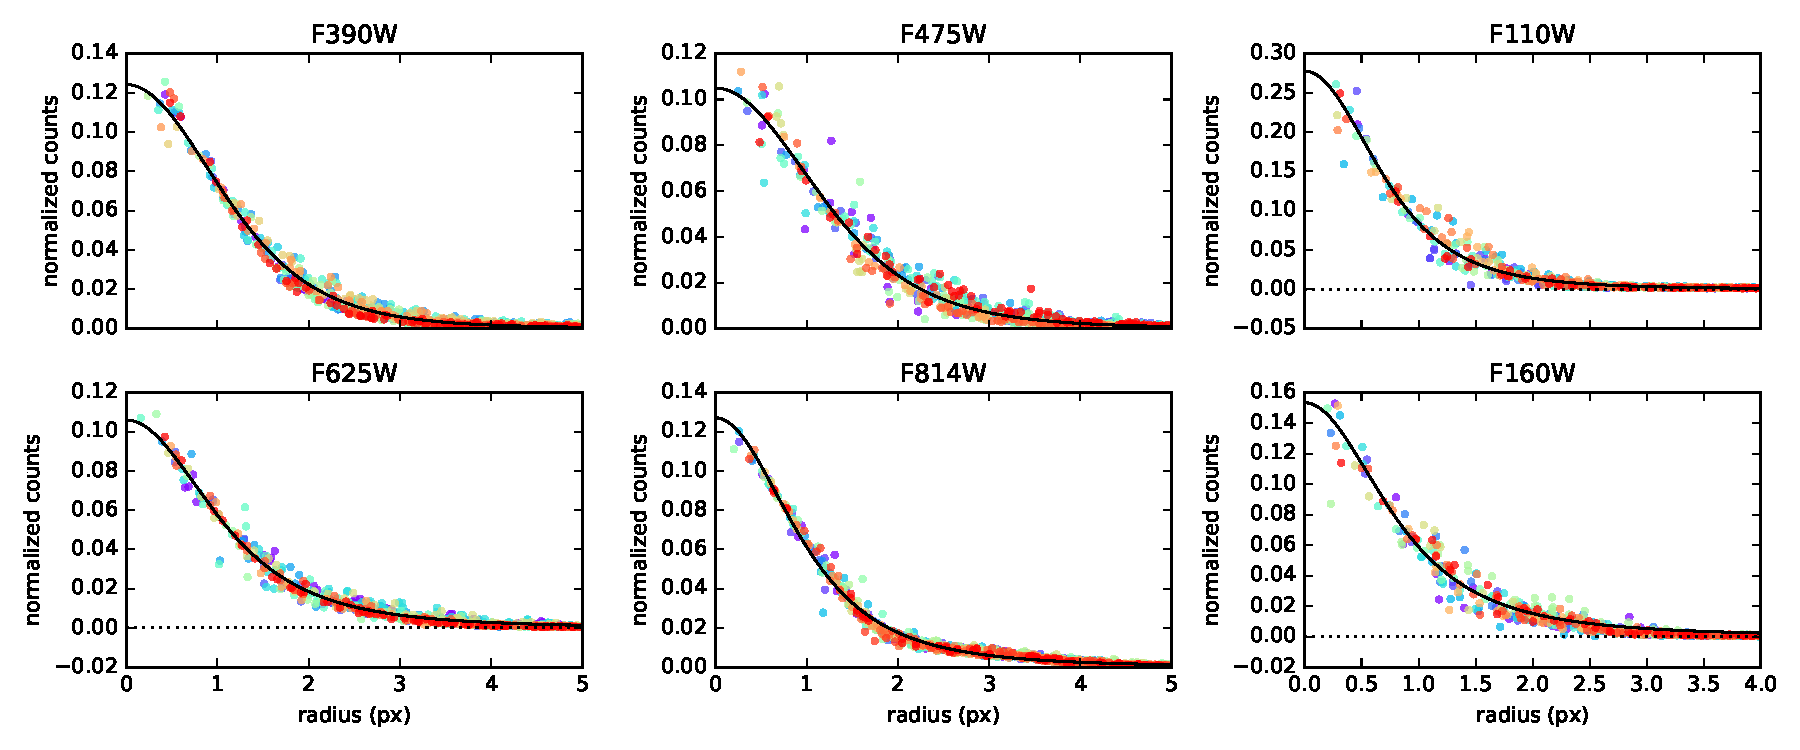
\includegraphics[width=\textwidth]{wfc3_psf_profiles.pdf}
%\caption{%
%	Stars observed between 2010 and 2017.  Each point shows the normalized pixel value for an individual observation of a star which
%	are represented by the different colors.  The fitted PSF amplitude for each star was used to normalized the pixel values.  The solid
%	lines show the fitted PSF profiles for each filter.
%	\label{fig:psf}
%}
%\end{figure*}

\begin{figure}
\centering
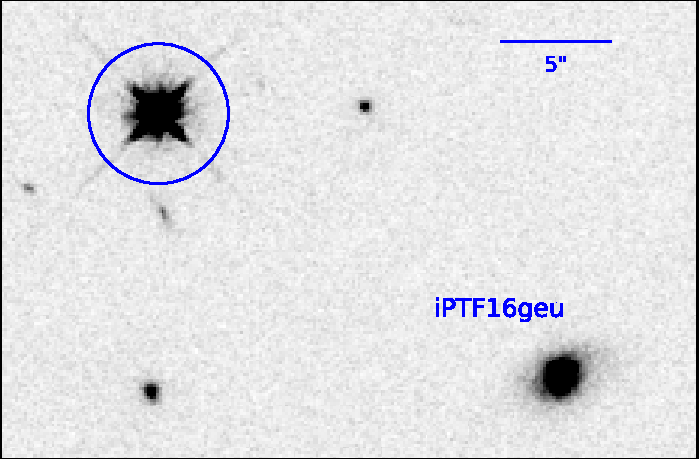
\includegraphics[width=\columnwidth]{psf_ir_star.pdf}
\caption{%
	Observation of \geu in the F110W band obtained on November 17th, 2016.  The blue circle marks the bright star visible in
	all IR observations, that was used for determining the aperture correction.
	\label{fig:psfnir}
}
\end{figure}


\section{Photometry of \geu}
Here we present the data tables that the the analysis in this paper is based on.

\begin{landscape}
\begin{table}
	\centering
	\caption{%
		Derived photometry for the four lensed \sn images.  The first error quoted for each measurement is the statistical
		uncertainty that is expected to uncorrelated between epochs.  This includes the expected PSF variations discussed
		in \S\ref{sec:wfcpsf}.  The second error, is the systematic error from the background model fit discussed in the text.
		This is will be correlated for measurements obtained with the same filter.
	\label{tb:resolvflux}}
	\begin{tabular}{r c r @{\hspace{0.5em}} l r @{\hspace{0.5em}} l r @{\hspace{0.5em}} l r @{\hspace{0.5em}} l r}
\hline\hline
\multicolumn{1}{c}{MJD} & \multicolumn{1}{c}{Filter} & \multicolumn{2}{c}{Flux \#1} & \multicolumn{2}{c}{Flux \#2} & \multicolumn{2}{c}{Flux \#3} & \multicolumn{2}{c}{Flux \#4} & \multicolumn{1}{c}{ZP}\\
\multicolumn{1}{c}{(days)} & & \multicolumn{2}{c}{(counts/s)} & \multicolumn{2}{c}{(counts/s)} & \multicolumn{2}{c}{(counts/s)} & \multicolumn{2}{c}{(counts/s)} & \multicolumn{1}{c}{(mag)}\\
\hline
57681.64 & $F110W$ & 5.17E$+$02 & (1E$+$01,1E$+$01) & 1.74E$+$02 & (8E$+$00,1E$+$01) & 1.02E$+$02 & (8E$+$00,2E$+$01) & 4.98E$+$01 & (9E$+$00,1E$+$01) & 26.64\\
57681.64 & $F160W$ & 1.21E$+$02 & (7E$+$00,5E$+$00) & 5.03E$+$01 & (5E$+$00,7E$+$00) & 3.59E$+$01 & (5E$+$00,7E$+$00) & 8.16E$+$00 & (6E$+$00,6E$+$00) & 25.76\\
57685.91 & $F625W$ & 5.58E$+$01 & (5E$+$00,2E$-$01) & 1.80E$+$01 & (2E$+$00,6E$-$01) & 5.64E$+$00 & (7E$-$01,6E$-$01) & 1.38E$+$00 & (5E$-$01,7E$-$01) & 25.42\\
57685.92 & $F814W$ & 1.15E$+$02 & (3E$+$00,0E$+$00) & 4.06E$+$01 & (1E$+$00,0E$+$00) & 1.29E$+$01 & (8E$-$01,4E$-$01) & 6.90E$+$00 & (7E$-$01,5E$-$01) & 24.99\\
57685.93 & $F475W$ & 8.44E$+$00 & (1E$+$00,0E$+$00) & 3.07E$+$00 & (5E$-$01,0E$+$00) & 7.50E$-$01 & (4E$-$01,0E$+$00) & $-$2.87E$-$01 & (4E$-$01,0E$+$00) & 25.58\\
57685.94 & $F390W$ & 5.67E$-$01 & (2E$-$01,0E$+$00) & 2.02E$-$01 & (2E$-$01,0E$+$00) & 3.54E$-$01 & (2E$-$01,0E$+$00) & $-$1.12E$-$01 & (2E$-$01,0E$+$00) & 25.24\\
57685.99 & $F110W$ & 4.15E$+$02 & (1E$+$01,1E$+$01) & 2.03E$+$02 & (9E$+$00,1E$+$01) & 1.26E$+$02 & (8E$+$00,1E$+$01) & 4.37E$+$01 & (9E$+$00,1E$+$01) & 26.64\\
57685.99 & $F160W$ & 1.21E$+$02 & (9E$+$00,0E$+$00) & 5.66E$+$01 & (6E$+$00,6E$+$00) & 4.67E$+$01 & (6E$+$00,6E$+$00) & 2.63E$+$00 & (7E$+$00,4E$+$00) & 25.76\\
57689.91 & $F625W$ & 4.09E$+$01 & (3E$+$00,6E$-$01) & 1.36E$+$01 & (1E$+$00,7E$-$01) & 4.27E$+$00 & (5E$-$01,7E$-$01) & 6.12E$-$01 & (4E$-$01,7E$-$01) & 25.42\\
57689.91 & $F814W$ & 9.39E$+$01 & (2E$+$00,4E$-$01) & 3.36E$+$01 & (1E$+$00,7E$-$01) & 9.43E$+$00 & (5E$-$01,8E$-$01) & 5.61E$+$00 & (5E$-$01,8E$-$01) & 24.99\\
57689.96 & $F110W$ & 5.20E$+$02 & (1E$+$01,1E$+$01) & 2.08E$+$02 & (9E$+$00,1E$+$01) & 1.05E$+$02 & (8E$+$00,2E$+$01) & 2.40E$+$01 & (9E$+$00,1E$+$01) & 26.64\\
57689.96 & $F160W$ & 1.90E$+$02 & (7E$+$00,5E$+$00) & 7.00E$+$01 & (5E$+$00,7E$+$00) & 4.06E$+$01 & (5E$+$00,7E$+$00) & $-$2.67E$+$00 & (6E$+$00,6E$+$00) & 25.76\\
57694.21 & $F625W$ & 3.44E$+$01 & (3E$+$00,7E$-$01) & 1.17E$+$01 & (1E$+$00,8E$-$01) & 3.83E$+$00 & (4E$-$01,8E$-$01) & 2.47E$-$01 & (2E$-$01,8E$-$01) & 25.42\\
57694.21 & $F814W$ & 8.70E$+$01 & (2E$+$00,6E$-$01) & 2.97E$+$01 & (8E$-$01,8E$-$01) & 9.43E$+$00 & (4E$-$01,8E$-$01) & 5.32E$+$00 & (4E$-$01,8E$-$01) & 24.99\\
57694.24 & $F110W$ & 5.97E$+$02 & (1E$+$01,1E$+$01) & 1.77E$+$02 & (8E$+$00,1E$+$01) & 9.54E$+$01 & (8E$+$00,2E$+$01) & 2.45E$+$01 & (9E$+$00,1E$+$01) & 26.64\\
57694.24 & $F160W$ & 2.34E$+$02 & (8E$+$00,2E$+$00) & 8.63E$+$01 & (6E$+$00,6E$+$00) & 4.13E$+$01 & (6E$+$00,6E$+$00) & 1.37E$+$01 & (7E$+$00,5E$+$00) & 25.76\\
57698.25 & $F625W$ & 2.92E$+$01 & (2E$+$00,7E$-$01) & 1.01E$+$01 & (9E$-$01,8E$-$01) & 3.49E$+$00 & (4E$-$01,8E$-$01) & 2.28E$-$01 & (3E$-$01,8E$-$01) & 25.42\\
57698.25 & $F814W$ & 7.15E$+$01 & (2E$+$00,6E$-$01) & 2.49E$+$01 & (7E$-$01,7E$-$01) & 7.29E$+$00 & (4E$-$01,8E$-$01) & 4.61E$+$00 & (4E$-$01,8E$-$01) & 24.99\\
57698.26 & $F110W$ & 4.60E$+$02 & (1E$+$01,1E$+$01) & 1.47E$+$02 & (8E$+$00,1E$+$01) & 8.85E$+$01 & (8E$+$00,2E$+$01) & 2.17E$+$01 & (9E$+$00,1E$+$01) & 26.64\\
57698.26 & $F160W$ & 2.04E$+$02 & (7E$+$00,5E$+$00) & 7.36E$+$01 & (5E$+$00,7E$+$00) & 4.45E$+$01 & (5E$+$00,7E$+$00) & 1.47E$+$01 & (6E$+$00,6E$+$00) & 25.76\\
57702.16 & $F625W$ & 1.74E$+$01 & (1E$+$00,8E$-$01) & 8.52E$+$00 & (8E$-$01,8E$-$01) & 2.90E$+$00 & (3E$-$01,8E$-$01) & 3.09E$-$01 & (2E$-$01,8E$-$01) & 25.42\\
57702.16 & $F814W$ & 6.03E$+$01 & (2E$+$00,7E$-$01) & 1.96E$+$01 & (6E$-$01,8E$-$01) & 6.81E$+$00 & (4E$-$01,8E$-$01) & 3.73E$+$00 & (4E$-$01,8E$-$01) & 24.99\\
57702.17 & $F110W$ & 3.24E$+$02 & (1E$+$01,1E$+$01) & 1.30E$+$02 & (8E$+$00,1E$+$01) & 8.54E$+$01 & (8E$+$00,2E$+$01) & 3.05E$+$01 & (9E$+$00,1E$+$01) & 26.64\\
57702.17 & $F160W$ & 1.75E$+$02 & (8E$+$00,2E$+$00) & 6.87E$+$01 & (6E$+$00,6E$+$00) & 3.72E$+$01 & (6E$+$00,6E$+$00) & 1.18E$+$01 & (7E$+$00,5E$+$00) & 25.76\\
57707.12 & $F625W$ & 1.87E$+$01 & (2E$+$00,7E$-$01) & 7.07E$+$00 & (7E$-$01,8E$-$01) & 3.13E$+$00 & (4E$-$01,8E$-$01) & $-$7.55E$-$02 & (3E$-$01,8E$-$01) & 25.42\\
57707.12 & $F814W$ & 4.97E$+$01 & (1E$+$00,7E$-$01) & 1.76E$+$01 & (6E$-$01,8E$-$01) & 5.74E$+$00 & (4E$-$01,8E$-$01) & 2.90E$+$00 & (4E$-$01,8E$-$01) & 24.99\\
57707.14 & $F110W$ & 2.89E$+$02 & (1E$+$01,1E$+$01) & 1.05E$+$02 & (8E$+$00,1E$+$01) & 7.37E$+$01 & (8E$+$00,2E$+$01) & 7.85E$+$00 & (9E$+$00,1E$+$01) & 26.64\\
57707.14 & $F160W$ & 1.33E$+$02 & (7E$+$00,4E$+$00) & 5.81E$+$01 & (5E$+$00,7E$+$00) & 3.78E$+$01 & (5E$+$00,7E$+$00) & 9.04E$+$00 & (6E$+$00,6E$+$00) & 25.76\\
57709.72 & $F625W$ & 2.15E$+$01 & (2E$+$00,7E$-$01) & 7.16E$+$00 & (7E$-$01,8E$-$01) & 2.74E$+$00 & (3E$-$01,8E$-$01) & $-$7.33E$-$02 & (2E$-$01,8E$-$01) & 25.42\\
57709.74 & $F814W$ & 4.72E$+$01 & (1E$+$00,7E$-$01) & 1.75E$+$01 & (6E$-$01,8E$-$01) & 5.32E$+$00 & (4E$-$01,8E$-$01) & 2.56E$+$00 & (4E$-$01,8E$-$01) & 24.99\\
57709.78 & $F110W$ & 1.94E$+$02 & (1E$+$01,1E$+$01) & 1.04E$+$02 & (8E$+$00,1E$+$01) & 7.79E$+$01 & (8E$+$00,2E$+$01) & 7.60E$+$00 & (9E$+$00,1E$+$01) & 26.64\\
57709.78 & $F160W$ & 1.19E$+$02 & (8E$+$00,2E$+$00) & 5.13E$+$01 & (6E$+$00,6E$+$00) & 3.57E$+$01 & (6E$+$00,6E$+$00) & 5.26E$+$00 & (7E$+$00,5E$+$00) & 25.76\\
57714.32 & $F625W$ & 2.02E$+$01 & (2E$+$00,7E$-$01) & 6.66E$+$00 & (6E$-$01,8E$-$01) & 2.84E$+$00 & (4E$-$01,8E$-$01) & 1.98E$-$01 & (3E$-$01,8E$-$01) & 25.42\\
57714.32 & $F814W$ & 4.19E$+$01 & (1E$+$00,7E$-$01) & 1.49E$+$01 & (5E$-$01,8E$-$01) & 4.98E$+$00 & (4E$-$01,8E$-$01) & 2.58E$+$00 & (4E$-$01,8E$-$01) & 24.99\\
\hline\hline
\end{tabular}

\end{table}
\end{landscape}

%%%%%%%%%%%%%%%%%%%%%%%%%%%%%%%%%%%%%%%%%%%%%%%%%%


% Don't change these lines
\bsp	% typesetting comment
\label{lastpage}
\end{document}

% End of mnras_template.tex